\documentclass[12pt,a4paper]{article}
\usepackage[left=2cm,right=2cm,top=2.5cm,bottom=2.5cm]{geometry}
\usepackage[utf8]{inputenc}
\usepackage[T1]{fontenc}
\usepackage{xcolor}
\usepackage{graphicx}
\usepackage{booktabs}
\usepackage{caption}
\usepackage{longtable}
\usepackage{hyperref}
\usepackage{geometry}
\usepackage{titlesec}
\usepackage{enumitem}

% Cores do tema cinza elegante
\definecolor{gray900}{RGB}{50,50,50}
\definecolor{gray700}{RGB}{80,80,80}
\definecolor{gray500}{RGB}{120,120,120}
\definecolor{gray300}{RGB}{200,200,200}
\definecolor{gray100}{RGB}{245,245,245}
\definecolor{accent}{RGB}{70,130,180}

% Configurações de hyperlink
\hypersetup{
    colorlinks=true,
    linkcolor=gray700,
    filecolor=gray700,
    urlcolor=accent,
    citecolor=gray700
}

% Título e seções
\titleformat{\section}{\Large\bfseries\color{gray900}}{\thesection}{1em}{}
\titleformat{\subsection}{\large\bfseries\color{gray700}}{\thesubsection}{1em}{}
\titleformat{\subsubsection}{\normalsize\bfseries\color{gray700}}{\thesubsubsection}{1em}{}

\titlespacing{\section}{0pt}{12pt}{6pt}
\titlespacing{\subsection}{0pt}{8pt}{4pt}
\titlespacing{\subsubsection}{0pt}{6pt}{2pt}

% Estilo das tabelas
\renewenvironment{table}%
{\begin{center}%
\scriptsize%
\addtolength{\tabcolsep}{-2pt}%
}%
{\end{center}}

\captionsetup{
    font=small,
    labelfont=bf,
    textfont=it,
    justification=raggedright
}

% Novo comando para tabela sem centro
\newenvironment{table*}%
{\begin{center}%
\addtolength{\tabcolsep}{-2pt}%
}%
{\end{center}}

% Capa
\begin{document}

%====================================================================
% CAPA
%====================================================================
\begin{titlepage}
\thispagestyle{empty}
%\pagecolor{gray100}

\vspace*{2cm}
\begin{center}
\Large\textbf{\color{gray900}\uppercase{Orçamento de Mão de Obra}}\\[0.5cm]
\Large\textbf{\color{gray900}\uppercase{Instalações Elétricas}}\\[1cm]

\vspace{2cm}

\Large\textbf{\color{gray700}\uppercase{Universidade Federal do Cariri -- UFCA}}\\[0.5cm]
\Large\textbf{\color{gray700}\uppercase{Bloco O}}

\vspace{3cm}

\begin{table}
\centering
\large
\begin{tabular}{p{3cm}p{8cm}}
\textbf{Projeto:} & Universidade Federal do Cariri - UFCA (Bloco O) \\
\textbf{Objetivo:} & Orçamento de mão de obra para instalações elétricas \\
\textbf{Referência:} & Projeto Elétrico - ELE.pdf \\
\textbf{Data:} & 27 de Março de 2026 \\
\textbf{Validade:} & 30 dias
\end{tabular}
\end{table}

\vfill

\begin{flushright}
\textbf{FEITOSA ENGENHARIA LTDA} \\
CNPJ: 58.554.143/0001-25 \\
Responsável: Francisco Cleber da Conceição Feitosa \\
CREA: 378933/CE
\end{flushright}

\vspace{2cm}

\end{titlepage}
\pagebreak

%====================================================================
% DADOS DA CONTRATADA
%====================================================================
\section{Dados da Contratada}

\begin{table}
\centering
\begin{tabular}{lp{10cm}}
\toprule
\textbf{Razão Social} & FEITOSA ENGENHARIA LTDA \\
\textbf{CNPJ} & 58.554.143/0001-25 \\
\textbf{Responsável Técnico} & Francisco Cleber da Conceição Feitosa \\
\textbf{CREA} & 378933/CE \\
\textbf{Telefone} & (88) 9.9999-9999 \\
\textbf{E-mail} & contato@feitosaengenharia.com.br \\
\textbf{Endereço} & Av. Padre Cícero, 123 - Juazeiro do Norte, CE \\
\bottomrule
\end{tabular}
\end{table}

\vspace{1cm}

%====================================================================
% RESUMO EXECUTIVO
%====================================================================
\section{Resumo Executivo}

\begin{table}
\centering
\begin{tabular}{clcc}
\toprule
\textbf{Item} & \textbf{Descrição} & \textbf{Quantidade} & \textbf{Und.} \\
\midrule
1 & Tomadas (total) & 263 & un \\
2 & Interruptores & 30 & un \\
3 & Disjuntores & 104 & un \\
4 & Eletrodutos 3/4'' & 4000 & m \\
5 & Fios/Cabos & 13900 & m \\
6 & Quadros distribuição & 8 & un \\
7 & Iluminação & 297 & un \\
8 & SPDA & 4.367,18 & R\$ \\
9 & Eletrocalhas & 240 & m \\
10 & RTA (pontos) & 141 & un \\
11 & RTA (cabo) & 2000 & m \\
12 & Bombas & 5 & un \\
13 & Quadros Comando & 4 & un \\
14 & Ilum. Externa (pontos) & 26 & un \\
15 & Ilum. Externa (cabo) & 1000 & m \\
16 & Ar Condicionado & 31 & un \\
\bottomrule
\end{tabular}
\end{table}

\pagebreak

%====================================================================
% 1. INSTALAÇÃO ELÉTRICA
%====================================================================
\section{1. Instalação Elétrica}

\subsection{1.1 Tomadas}

\begin{table}
\centering
\begin{tabular}{lccccr}
\toprule
\textbf{Item} & \textbf{Descrição} & \textbf{Código SINAPI} & \textbf{Qtd} & \textbf{Custo MO/Un} & \textbf{Total MO (R\$)} \\
\midrule
1.1 & Tomada alta 2P+T 10A & 91990 & 29 & 16,31 & 473,00 \\
1.2 & Tomada média 2P+T 10A & 91994 & 9 & 10,12 & 91,08 \\
1.3 & Tomada baixa 2P+T 10A & 91998 & 225 & 7,72 & 1.737,00 \\
\midrule
 & \textbf{Subtotal Tomadas} & & 263 & & \textbf{2.301,08} \\
\bottomrule
\end{tabular}
\end{table}

\subsection{1.2 Interruptores}

\begin{table}
\centering
\begin{tabular}{lccccr}
\toprule
\textbf{Item} & \textbf{Descrição} & \textbf{Código SINAPI} & \textbf{Qtd} & \textbf{Custo MO/Un} & \textbf{Total MO (R\$)} \\
\midrule
1.4 & Interruptor simples 1 tecla & 91940 & 30 & 9,42 & 282,60 \\
\midrule
 & \textbf{Subtotal Interruptores} & & 30 & & \textbf{282,60} \\
\bottomrule
\end{tabular}
\end{table}

\subsection{1.3 Disjuntores}

\begin{table}
\centering
\begin{tabular}{lp{4.5cm}cccr}
\toprule
\textbf{Quadro} & \textbf{Tipo} & \textbf{Qtd} & \textbf{Custo MO/Un} & \textbf{Total (R\$)} \\
\midrule
QLF-T & Disjuntor TRIFÁSICO 100A & 1 & 18,09 & 18,09 \\
QLF-T & Disjuntor TRIFÁSICO 63A & 1 & 18,09 & 18,09 \\
QLF-T & DPS MONO 275V & 4 & 15,00* & 60,00 \\
QLF-T & Disjuntor MONO 20A & 25 & 2,10 & 52,50 \\
QLF-T & Disjuntor MONO 16A & 4 & 1,49 & 5,96 \\
\midrule
QLF-S & Disjuntor TRIFÁSICO 80A & 1 & 18,09 & 18,09 \\
QLF-S & Disjuntor TRIFÁSICO 63A & 1 & 18,09 & 18,09 \\
QLF-S & DPS MONO 275V & 4 & 15,00* & 60,00 \\
QLF-S & Disjuntor MONO 20A & 19 & 2,10 & 39,90 \\
QLF-S & Disjuntor MONO 16A & 4 & 1,49 & 5,96 \\
\midrule
QFAC-T & Disjuntor TRIFÁSICO 125A & 1 & 18,09 & 18,09 \\
QFAC-T & Disjuntor TRIFÁSICO 63A & 1 & 18,09 & 18,09 \\
QFAC-T & DPS MONO 275V & 4 & 15,00* & 60,00 \\
QFAC-T & Disjuntor MONO 32A & 10 & 2,90 & 29,00 \\
QFAC-T & Disjuntor MONO 25A & 10 & 2,10 & 21,00 \\
\midrule
QFAC-S & Disjuntor TRIFÁSICO 100A & 1 & 18,09 & 18,09 \\
QFAC-S & Disjuntor TRIFÁSICO 63A & 1 & 18,09 & 18,09 \\
QFAC-S & DPS MONO 275V & 4 & 15,00* & 60,00 \\
QFAC-S & Disjuntor MONO 32A & 11 & 2,90 & 31,90 \\
QFAC-S & Disjuntor MONO 20A & 8 & 2,10 & 16,80 \\
\midrule
Bombas & Disjuntor MONO 16A & 3 & 1,49 & 4,47 \\
Bombas & Disjuntor MONO 50A & 1 & 6,03 & 6,03 \\
\midrule
 & \textbf{Subtotal Disjuntores} & 104 & & \textbf{598,24} \\
\bottomrule
\end{tabular}
\end{table}

\noindent\small{*Valor estimado para DPS}

\subsection{1.4 Eletrodutos}

\begin{table}
\centering
\begin{tabular}{lccccr}
\toprule
\textbf{Item} & \textbf{Descrição} & \textbf{Código SINAPI} & \textbf{Qtd} & \textbf{Custo MO/Un} & \textbf{Total MO (R\$)} \\
\midrule
1.4.1 & Eletroduto PVC 3/4'' (parede) & 91854 & 4000 & 4,29 & 17.160,00 \\
\midrule
 & \textbf{Subtotal Eletrodutos} & & 4000m & & \textbf{17.160,00} \\
\bottomrule
\end{tabular}
\end{table}

\subsubsubsection{1.4.1 Cortes em Alvenaria (Passagem Eletrodutos)}

\noindent\textbf{Metodologia:} Comprimento calculado pela altura relativa ao forro (2,7m):
\begin{itemize}
    \item Tomadas baixas (h=0,30m): 2,4m por ponto
    \item Demais pontos (h=1,10m): 1,6m por ponto
\end{itemize}

\begin{table}
\centering
\begin{tabular}{lccccr}
\toprule
\textbf{Item} & \textbf{Descrição} & \textbf{Código SINAPI} & \textbf{Qtd} & \textbf{Custo MO/Un} & \textbf{Total MO (R\$)} \\
\midrule
1.4.1.1 & Rasgo linear em alvenaria (eletrodutos $\leq$40mm) & 90447 & 875 & 12,65 & 11.068,75 \\
1.4.1.2 & Quebra em alvenaria p/ caixa 4x2 & 90456 & 405 & 8,39 & 3.397,95 \\
1.4.1.3 & Chumbamento linear em alvenaria (eletrodutos $\leq$40mm) & 104766 & 438 & 22,48 & 9.846,24 \\
1.4.1.4 & Chumbamento de caixas 4x2 (fixação) & 91940* & 405 & 12,00 & 4.860,00 \\
\midrule
 & \textbf{Subtotal Cortes Alvenaria} & & & & \textbf{29.172,94} \\
\bottomrule
\end{tabular}
\end{table}

\noindent\small{*MO estimada (composição 91940 inclui apenas fixação básica)}
\noindent\small{*Base SINAPI 11/2025 - Custo não desonerado}

\subsection{1.5 Fios e Cabos}

\begin{table}
\centering
\begin{tabular}{lcccr}
\toprule
\textbf{Item} & \textbf{Descrição} & \textbf{Qtd} & \textbf{Custo MO/Un*} & \textbf{Total MO (R\$)} \\
\midrule
1.6 & Fio/Cabo 2,5mm² & 10000 & 0,73 & 7.300,00 \\
1.7 & Fio/Cabo 4mm² & 2000 & 0,73 & 1.460,00 \\
1.8 & Fio/Cabo 6mm² & 1000 & 0,73 & 730,00 \\
1.9 & Fio/Cabo 10mm² & 500 & 0,73 & 365,00 \\
1.10 & Fio/Cabo 16mm² & 200 & 0,73 & 146,00 \\
1.11 & Cabo nu aterramento & 200 & 0,73 & 146,00 \\
\midrule
 & \textbf{Subtotal Fios/Cabos} & 13900m & & \textbf{10.147,00} \\
\bottomrule
\end{tabular}
\end{table}

\noindent\small{*Valor estimado baseado em composição SINAPI 91924}

\pagebreak

\subsection{1.6 Quadros}

\begin{table}
\centering
\begin{tabular}{lccccr}
\toprule
\textbf{Item} & \textbf{Descrição} & \textbf{Código SINAPI} & \textbf{Qtd} & \textbf{Custo MO/Un} & \textbf{Total MO (R\$)} \\
\midrule
1.12 & Quadro distribuição & 101876 & 8 & 10,98 & 87,84 \\
\midrule
 & \textbf{Subtotal Quadros} & & 8 & & \textbf{87,84} \\
\bottomrule
\end{tabular}
\end{table}

\subsection{1.7 Iluminação}

\begin{table}
\centering
\begin{tabular}{lcccr}
\toprule
\textbf{Item} & \textbf{Descrição} & \textbf{Qtd} & \textbf{Custo MO/Un*} & \textbf{Total MO (R\$)} \\
\midrule
1.13 & Luminária LED 18Wx2 & 297 & 5,00 & 1.485,00 \\
\midrule
 & \textbf{Subtotal Iluminação} & 297 & & \textbf{1.485,00} \\
\bottomrule
\end{tabular}
\end{table}

\noindent\small{*Valor estimado}

%====================================================================
% 2. SPDA
%====================================================================
\section{2. SPDA}

\subsection{2.1 Aterramento (Malha)}

\begin{table}
\centering
\begin{tabular}{lccccr}
\toprule
\textbf{Item} & \textbf{Descrição} & \textbf{Código SINAPI} & \textbf{Qtd} & \textbf{Custo MO/Un} & \textbf{Total MO (R\$)} \\
\midrule
2.1.1 & Haste aterramento cobre Ø5/8'' x 3m & 96985 & 14 & 5,87 & 82,18 \\
2.1.2 & Cordoalha cobre nu 50mm² (enterrada) & 96977 & 150 & 7,58 & 1.137,00 \\
2.1.3 & Solda exotérmica cabo-haste* & -- & 14 & 15,00 & 210,00 \\
\midrule
 & \textbf{Subtotal Aterramento} & & & & \textbf{1.429,18} \\
\bottomrule
\end{tabular}
\end{table}

\subsection{2.2 Captação (Malha Superior - Cobertura)}

\begin{table}
\centering
\begin{tabular}{lccccr}
\toprule
\textbf{Item} & \textbf{Descrição} & \textbf{Código SINAPI} & \textbf{Qtd} & \textbf{Custo MO/Un} & \textbf{Total MO (R\$)} \\
\midrule
2.2.1 & Barra chata alumínio 70mm² (7/8'' x 1/8'') c/ furos 7mm & 96980 & 180 & 7,58 & 1.364,40 \\
2.2.2 & Suporte isolador fixação alvenaria/concreto & 98463 & 60 & 2,45 & 147,00 \\
2.2.3 & Presilha fixação cordoalha & 104747 & 180 & 1,87 & 336,60 \\
\midrule
 & \textbf{Subtotal Captação} & & & & \textbf{1.848,00} \\
\bottomrule
\end{tabular}
\end{table}

\subsection{2.3 Descidas (Vergalhão REBAR Ø10mm)}

\begin{table}
\centering
\begin{tabular}{lccccr}
\toprule
\textbf{Item} & \textbf{Descrição} & \textbf{Código SINAPI} & \textbf{Qtd} & \textbf{Custo MO/Un} & \textbf{Total MO (R\$)} \\
\midrule
2.3.1 & Vergalhão aço Ø10mm (descida)* & -- & 200 & 5,00 & 1.000,00 \\
2.3.2 & Presilha fixação vergalhão* & -- & 60 & 1,50 & 90,00 \\
\midrule
 & \textbf{Subtotal Descidas} & & & & \textbf{1.090,00} \\
\bottomrule
\end{tabular}
\end{table}

\noindent\textbf{Subtotal SPDA (Mão de Obra):} \textbf{4.367,18}

\noindent\small{*Soldas exotérmicas: serviço especializado sem código SINAPI específico - valor estimado}
\noindent\small{*Vergalhão descida: serviço especializado sem código SINAPI específico - valor estimado}

\pagebreak

%====================================================================
% 3. CABEAMENTO ESTRUTURADO (RTA)
%====================================================================
\section{3. Cabeamento Estruturado (RTA)}

\begin{table}
\centering
\begin{tabular}{lcccr}
\toprule
\textbf{Item} & \textbf{Descrição} & \textbf{Qtd} & \textbf{Custo MO/Un*} & \textbf{Total MO (R\$)} \\
\midrule
3.1 & Ponto rede RJ45 & 141 & 15,00 & 2.115,00 \\
3.2 & Cabo rede Cat6 & 2000 & 0,50 & 1.000,00 \\
3.3 & Rack & 2 & 50,00 & 100,00 \\
\midrule
 & \textbf{Subtotal RTA} & & & \textbf{3.215,00} \\
\bottomrule
\end{tabular}
\end{table}

\noindent\small{*Valores estimados}

%====================================================================
% 4. BOMBAS E EQUIPAMENTOS
%====================================================================
\section{4. Bombas e Equipamentos}

\begin{table}
\centering
\begin{tabular}{lcccr}
\toprule
\textbf{Item} & \textbf{Descrição} & \textbf{Qtd} & \textbf{Custo MO/Un*} & \textbf{Total MO (R\$)} \\
\midrule
4.1 & Bomba centrífuga & 5 & 80,00 & 400,00 \\
4.2 & Quadro de comando & 4 & 60,00 & 240,00 \\
\midrule
 & \textbf{Subtotal Bombas} & & & \textbf{640,00} \\
\bottomrule
\end{tabular}
\end{table}

\noindent\small{*Valores estimados}

%====================================================================
% 5. ILUMINAÇÃO EXTERNA
%====================================================================
\section{5. Iluminação Externa}

\begin{table}
\centering
\begin{tabular}{lcccr}
\toprule
\textbf{Item} & \textbf{Descrição} & \textbf{Qtd} & \textbf{Custo MO/Un*} & \textbf{Total MO (R\$)} \\
\midrule
5.1 & Refletor LED 150W & 9 & 15,00 & 135,00 \\
5.2 & Poste 12m c/ 2 LED & 10 & 100,00 & 1.000,00 \\
5.3 & Poste 14m c/ 2 LED & 6 & 120,00 & 720,00 \\
5.4 & Cabo iluminação ext. & 1000 & 0,73 & 730,00 \\
5.5 & Quadro c/ temporizador & 1 & 80,00 & 80,00 \\
\midrule
 & \textbf{Subtotal Ilum. Ext.} & & & \textbf{2.665,00} \\
\bottomrule
\end{tabular}
\end{table}

\noindent\small{*Valores estimados}

%====================================================================
% 6. AR CONDICIONADO
%====================================================================
\section{6. Ar Condicionado}

\begin{table}
\centering
\begin{tabular}{lcccr}
\toprule
\textbf{Item} & \textbf{Descrição} & \textbf{Qtd} & \textbf{Custo MO/Un*} & \textbf{Total MO (R\$)} \\
\midrule
6.1 & Caixa passagem AC & 31 & 25,00 & 775,00 \\
\midrule
 & \textbf{Subtotal AC} & & & \textbf{775,00} \\
\bottomrule
\end{tabular}
\end{table}

\noindent\small{*Valor estimado}

\pagebreak

%====================================================================
% RESUMO ORÇAMENTO MÃO DE OBRA
%====================================================================
\section{Resumo Orçamento Mão de Obra}

\begin{table}
\centering
\begin{tabular}{clcr}
\toprule
\textbf{Item} & \textbf{Descrição} & \textbf{Total Mão de Obra (R\$)} \\
\midrule
1 & Tomadas & 2.301,08 \\
2 & Interruptores & 282,60 \\
3 & Disjuntores & 508,24 \\
4 & Eletrodutos (+ Cortes) & 46.332,94 \\
5 & Fios/Cabos & 10.147,00 \\
6 & Quadros & 87,84 \\
7 & Iluminação & 1.485,00 \\
8 & SPDA & 4.367,18 \\
9 & RTA & 3.215,00 \\
10 & Bombas/Comando & 640,00 \\
11 & Iluminação Externa & 2.665,00 \\
12 & Ar Condicionado & 775,00 \\
\midrule
 & \textbf{TOTAL MÃO DE OBRA} & \textbf{72.806,88} \\
\bottomrule
\end{tabular}
\end{table}

%====================================================================
% NOTA DE EXCLUSÕES
%====================================================================
\section{Nota de Exclusões}

\noindent\textbf{IMPORTANTE:} O presente orçamento refere-se EXCLUSIVAMENTE à mão de obra de instalações elétricas. NÃO estão incluidos nos serviços sob responsabilidade da contratada as seguintes atividades:

\begin{enumerate}[noitemsep]
\item \textbf{Escavações} -- Não inclusas; execução por conta da contratante
\item \textbf{Cortes em alvenaria} -- \textbf{INCLUSOS} (ver item 1.4.1)
\item \textbf{Instalações de subestações áreas ou cobertas} -- Não inclusas; execução por conta da contratante
\item \textbf{Construção de elementos de alvenaria} -- Não inclusos; execução por conta da contratante
\item \textbf{Caixas de passagem (eletrodutos em geral)} -- Estas devem ser executadas por pedreiros/serventes contratados pela parte contratante
\end{enumerate}

\pagebreak

%====================================================================
% COMPOSIÇÃO DA EQUIPE DE TRABALHO
%====================================================================
\section{Composição da Equipe de Trabalho}

O presente orçamento contempla a contratação de \textbf{três profissionais}:

\begin{table}
\centering
\begin{tabular}{lp{10cm}}
\toprule
\textbf{Profissional} & \textbf{Função / Atribuições} \\
\midrule
\textbf{Eletricista} & Execução técnica, montagem de eletrodutos, cabeamento, instalação de tomadas, interruptores, disjuntores, quadros, SPDA, RTA, iluminação, comissionamento \\
\midrule
\textbf{Pedreiro} & Cortes em alvenaria (rasgos, quebras), chumbamentos, fixações em alvenaria/concreto \\
\midrule
\textbf{Ajudante} & Auxiliar -- Transporte horizontal de materiais no andar de execução, suporte ao eletricista e pedreiro, preparação de materiais \\
\bottomrule
\end{tabular}
\end{table}

%====================================================================
% OBSERVAÇÕES TÉCNICAS
%====================================================================
\section{Observações Técnicas -- Aferição e Execução}

\subsection{Aferição (Levantamento de Produtividade)}

Para o levantamento dos índices de produtividade foi considerado que:

\begin{itemize}
\item \textbf{O ajudante é responsável também pelo transporte horizontal do material no andar de execução;}
\item \textbf{Foi considerado esforço de fixação provisória da instalação (feita em pontos localizados para montagem do eletroduto);}
\item \textbf{As produtividades desta composição não contemplam as seguintes atividades:}
\begin{itemize}
\item Fixações finais dos eletrodutos;
\item Fixação de abraçadeiras passantes em lajes;
\item Rasgos e cortes;
\item Chumbamentos.
\end{itemize}
\end{itemize}

\noindent\underline{Para tais atividades, utilizar composição específica de cada serviço.}

\subsection{Execução}

O processo de execução segue os seguintes passos:

\begin{enumerate}
\item \textbf{Verifica-se o comprimento do trecho da instalação;}
\item \textbf{Corta-se o comprimento necessário da bobina do eletroduto;}
\item \textbf{Fixa-se o eletroduto no local definido através de abraçadeiras} (os esforços de fixação das abraçadeiras não estão contemplados nesta composição);
\item \textbf{As extremidades são deixadas livres para posterior conexão.}
\end{enumerate}

\pagebreak

%====================================================================
% CRONOGRAMA DE EXECUÇÃO E DEPENDÊNCIAS
%====================================================================
\section{Cronograma de Execução e Dependências}

A execução das instalações elétricas segue uma ordem de dependência que respeita o avanço da obra civil. Abaixo, apresentamos a sequência recomendada:

\begin{table}
\centering
\begin{tabular}{cllcr}
\toprule
\textbf{Fase} & \textbf{Etapa} & \textbf{Serviço} & \textbf{Dependência} \\
\midrule
 & 1.1 & Eletrodutos (3/4'') - 4000m & Alvenaria completa \\
 & 1.2 & Eletrocalhas - 240m & Estrutura/laje pronta \\
 & 1.3 & Caixa passagem AC - 31un & Alvenaria em execução \\
\midrule
 & 2.1 & Fios e Cabos - 13900m & Eletrodutos finalizados \\
 & 2.2 & Cabo rede Cat6 - 2000m & Eletrocalhas instaladas \\
 & 2.3 & Cabo aterramento - 200m & Eletrodutos finalizados \\
\midrule
 & 3.1 & Tomadas - 263un & Alvenaria rebocada \\
 & 3.2 & Interruptores - 30un & Alvenaria rebocada \\
 & 3.3 & Disjuntores - 104un & Quadros instalados \\
 & 3.4 & Quadros distribuição - 8un & Eletrodutos finalizados \\
 & 3.5 & SPDA - 14un & 4.367,18 & Cobertura concretada \\
 & 3.6 & Pontos RTA - 141un & Alvenaria rebocada \\
\midrule
 & 4.1 & Iluminação - 297un & Fase 3 completa \\
 & 4.2 & Quadros comando - 4un & Bombas instaladas \\
 & 4.3 & Iluminação Externa - 26un & Postes instalados \\
 & 4.4 & Bombas - 5un & Hidráulica completa \\
\bottomrule
\end{tabular}
\end{table}

%====================================================================
% OPÇÕES DE PAGAMENTO
%====================================================================
\section{Opções de Pagamento}

\subsection{Opção 1: Pagamento por Medições (Recomendado)}

O pagamento será realizado conforme o avanço físico das etapas, mediante medições mensais aprovadas pela fiscalização.

\begin{table}
\centering
\begin{tabular}{ccccr}
\toprule
\textbf{Medição} & \textbf{Etapa} & \textbf{Período} & \textbf{Valor (R\$)} & \textbf{\% do Total} \\
\midrule
0 & \textbf{Sinal (Assinatura)} & -- & 5.104,24 & 10\% \\
1 & Fase 1 - Instalação Bruta & Mês 1 & 22.969,08 & 45\% \\
2 & Fase 2 - Cabeamento & Mês 2 & 14.814,00 & 29\% \\
3 & Fase 3 - Instalação Terminada & Mês 3 & 7.200,96 & 14\% \\
4 & Fase 4 - Comissionamento & Mês 4 & 1.029,28 & 2\% \\
\midrule
 & & \textbf{TOTAL COM DESCONTO} & \textbf{50.964,82} & \textbf{100\%} \\
 & Desconto appliqué (30\%) & & -21.842,06 & \\
\bottomrule
\end{tabular}
\end{table}

\noindent\textbf{Condições:}
\begin{itemize}
\item \textbf{10\% (R\$ 5.104,24) no ato da assinatura} -- para viabilizar custos iniciais (materiais, deslocamento, equipe) \textbf{E MARCAÇÃO DOS PONTOS necessários para as primeiras atividades}
\item Medições realizadas a cada 30 dias
\item Prazo de pagamento: até 15 dias após aprovação da medição
\item Retenção de 5\% até a conclusão final
\end{itemize}

\pagebreak

\subsection{Opção 2: Pagamento Mensal Fixo (5 Meses)}

Pagamento fixo mensal durante a execução da obra, independente do avanço físico.

\begin{table}
\centering
\begin{tabular}{ccr}
\toprule
\textbf{Mês} & \textbf{Descrição} & \textbf{Valor (R\$)} \\
\midrule
0 & \textbf{Sinal (Assinatura)} & 5.104,24 \\
1 & Início + Fase 1 & 22.969,08 \\
2 & Fase 2 & 10.156,33 \\
3 & Fase 3 & 7.200,96 \\
4 & Fase 4 parte 1 & 3.531,76 \\
5 & Fase 4 parte 2 + Saldo & 8.084,20 \\
\midrule
 & \textbf{TOTAL COM DESCONTO} & \textbf{50.964,82} \\
 & Desconto appliqué (30\%) & -21.842,06 \\
\bottomrule
\end{tabular}
\end{table}

\noindent\textbf{Condições:}
\begin{itemize}
\item \textbf{10\% (R\$ 5.104,24) no ato da assinatura} -- para viabilizar custos iniciais \textbf{E MARCAÇÃO DOS PONTOS necessários para as primeiras atividades}
\item Pagamento no 5º dia útil de cada mês
\item Primeiro pagamento no início da obra
\item Última parcela mediante aceite final
\end{itemize}

\pagebreak

%====================================================================
% DESCONTO POR PARCERIA
%====================================================================
\section{Desconto por Parceria}

\subsection{Condição Especial de Pagamento}

\textbf{Desconto de 30\%} válido para assinatura do contrato em até \textbf{5 dias} a contar da data de recebimento desta proposta.

\noindent\textit{O valor do desconto (R\$ 21.842,06) será distribuído proporcionalmente entre as fases/medições conforme opção de pagamento escolhida.}

\noindent\textbf{Valor com desconto: R\$ 50.964,82}

\noindent\textbf{Condições do desconto:}
\begin{itemize}
\item \textbf{10\% (R\$ 5.104,24) no ato da assinatura} -- para viabilizar custos iniciais E MARCAÇÃO DOS PONTOS necessários para as primeiras atividades
\item Restante conforme cronograma de execução
\item Assinatura do contrato em até 5 dias úteis
\item Pagamento único antecipado OU primeira parcela no ato da assinatura
\item Não cumulativo com outras promoções
\end{itemize}

\subsection{Resumo das Opções de Pagamento}

\begin{table}
\centering
\begin{tabular}{cccc}
\toprule
\textbf{Opção} & \textbf{Forma} & \textbf{Valor Total} & \textbf{Condição} \\
\midrule
1 & Medições & R\$ 72.806,88 & Conforme avanço \\
2 & Mensal 5x & R\$ 72.806,88 & R\$ 14.561,38/mês \\
\textbf{Com Desconto} & Única/Mensal & \textbf{R\$ 50.964,82} & Assinatura $\leq$ 5 dias \\
\bottomrule
\end{tabular}
\end{table}

\noindent\textit{Em caso de optar pela oportunidade do desconto, o valor reduzido (R\$ 21.842,06) será distribuído entre as fases/medições proporcionalmente ao percentual de cada etapa.}

\pagebreak

%====================================================================
% OBSERVAÇÕES FINAIS
%====================================================================
\section{Observações Finais}

\begin{itemize}
\item Os valores acima são baseados exclusivamente no custo de MÃO DE OBRA conforme composição SINAPI
\item Valores marcados com * são estimados -- recomenda-se verificar composição SINAPI específica
\end{itemize}

%====================================================================
% FÓRMULA DE CÁLCULO
%====================================================================
\section{Fórmula de Cálculo}

\begin{center}
\fbox{
\parbox{0.9\textwidth}{
\textbf{Mão de Obra Total} = $\Sigma$ (Quantidade $\times$ Custo Mão de Obra SINAPI)

\textbf{Orçamento Final} = Mão de Obra Total $\times$ (1 + BDI/100) + Materiais
}
}
\end{center}

\vfill

\noindent\textit{Dados extraídos das páginas 1, 2, 4, 5, 6, 8, 9, 10, 11, 13 do projeto ELE.pdf}
\par\noindent\textit{Orçamento gerado em 27/03/2026}

\pagebreak

%====================================================================
% ANEXO - PLANTAS MARCADAS
%====================================================================
\section{Anexo -- Plantas Marcadas do Projeto}

\subsection{Planta Página 1 - Térreo}
\begin{figure}[h!]
\centering
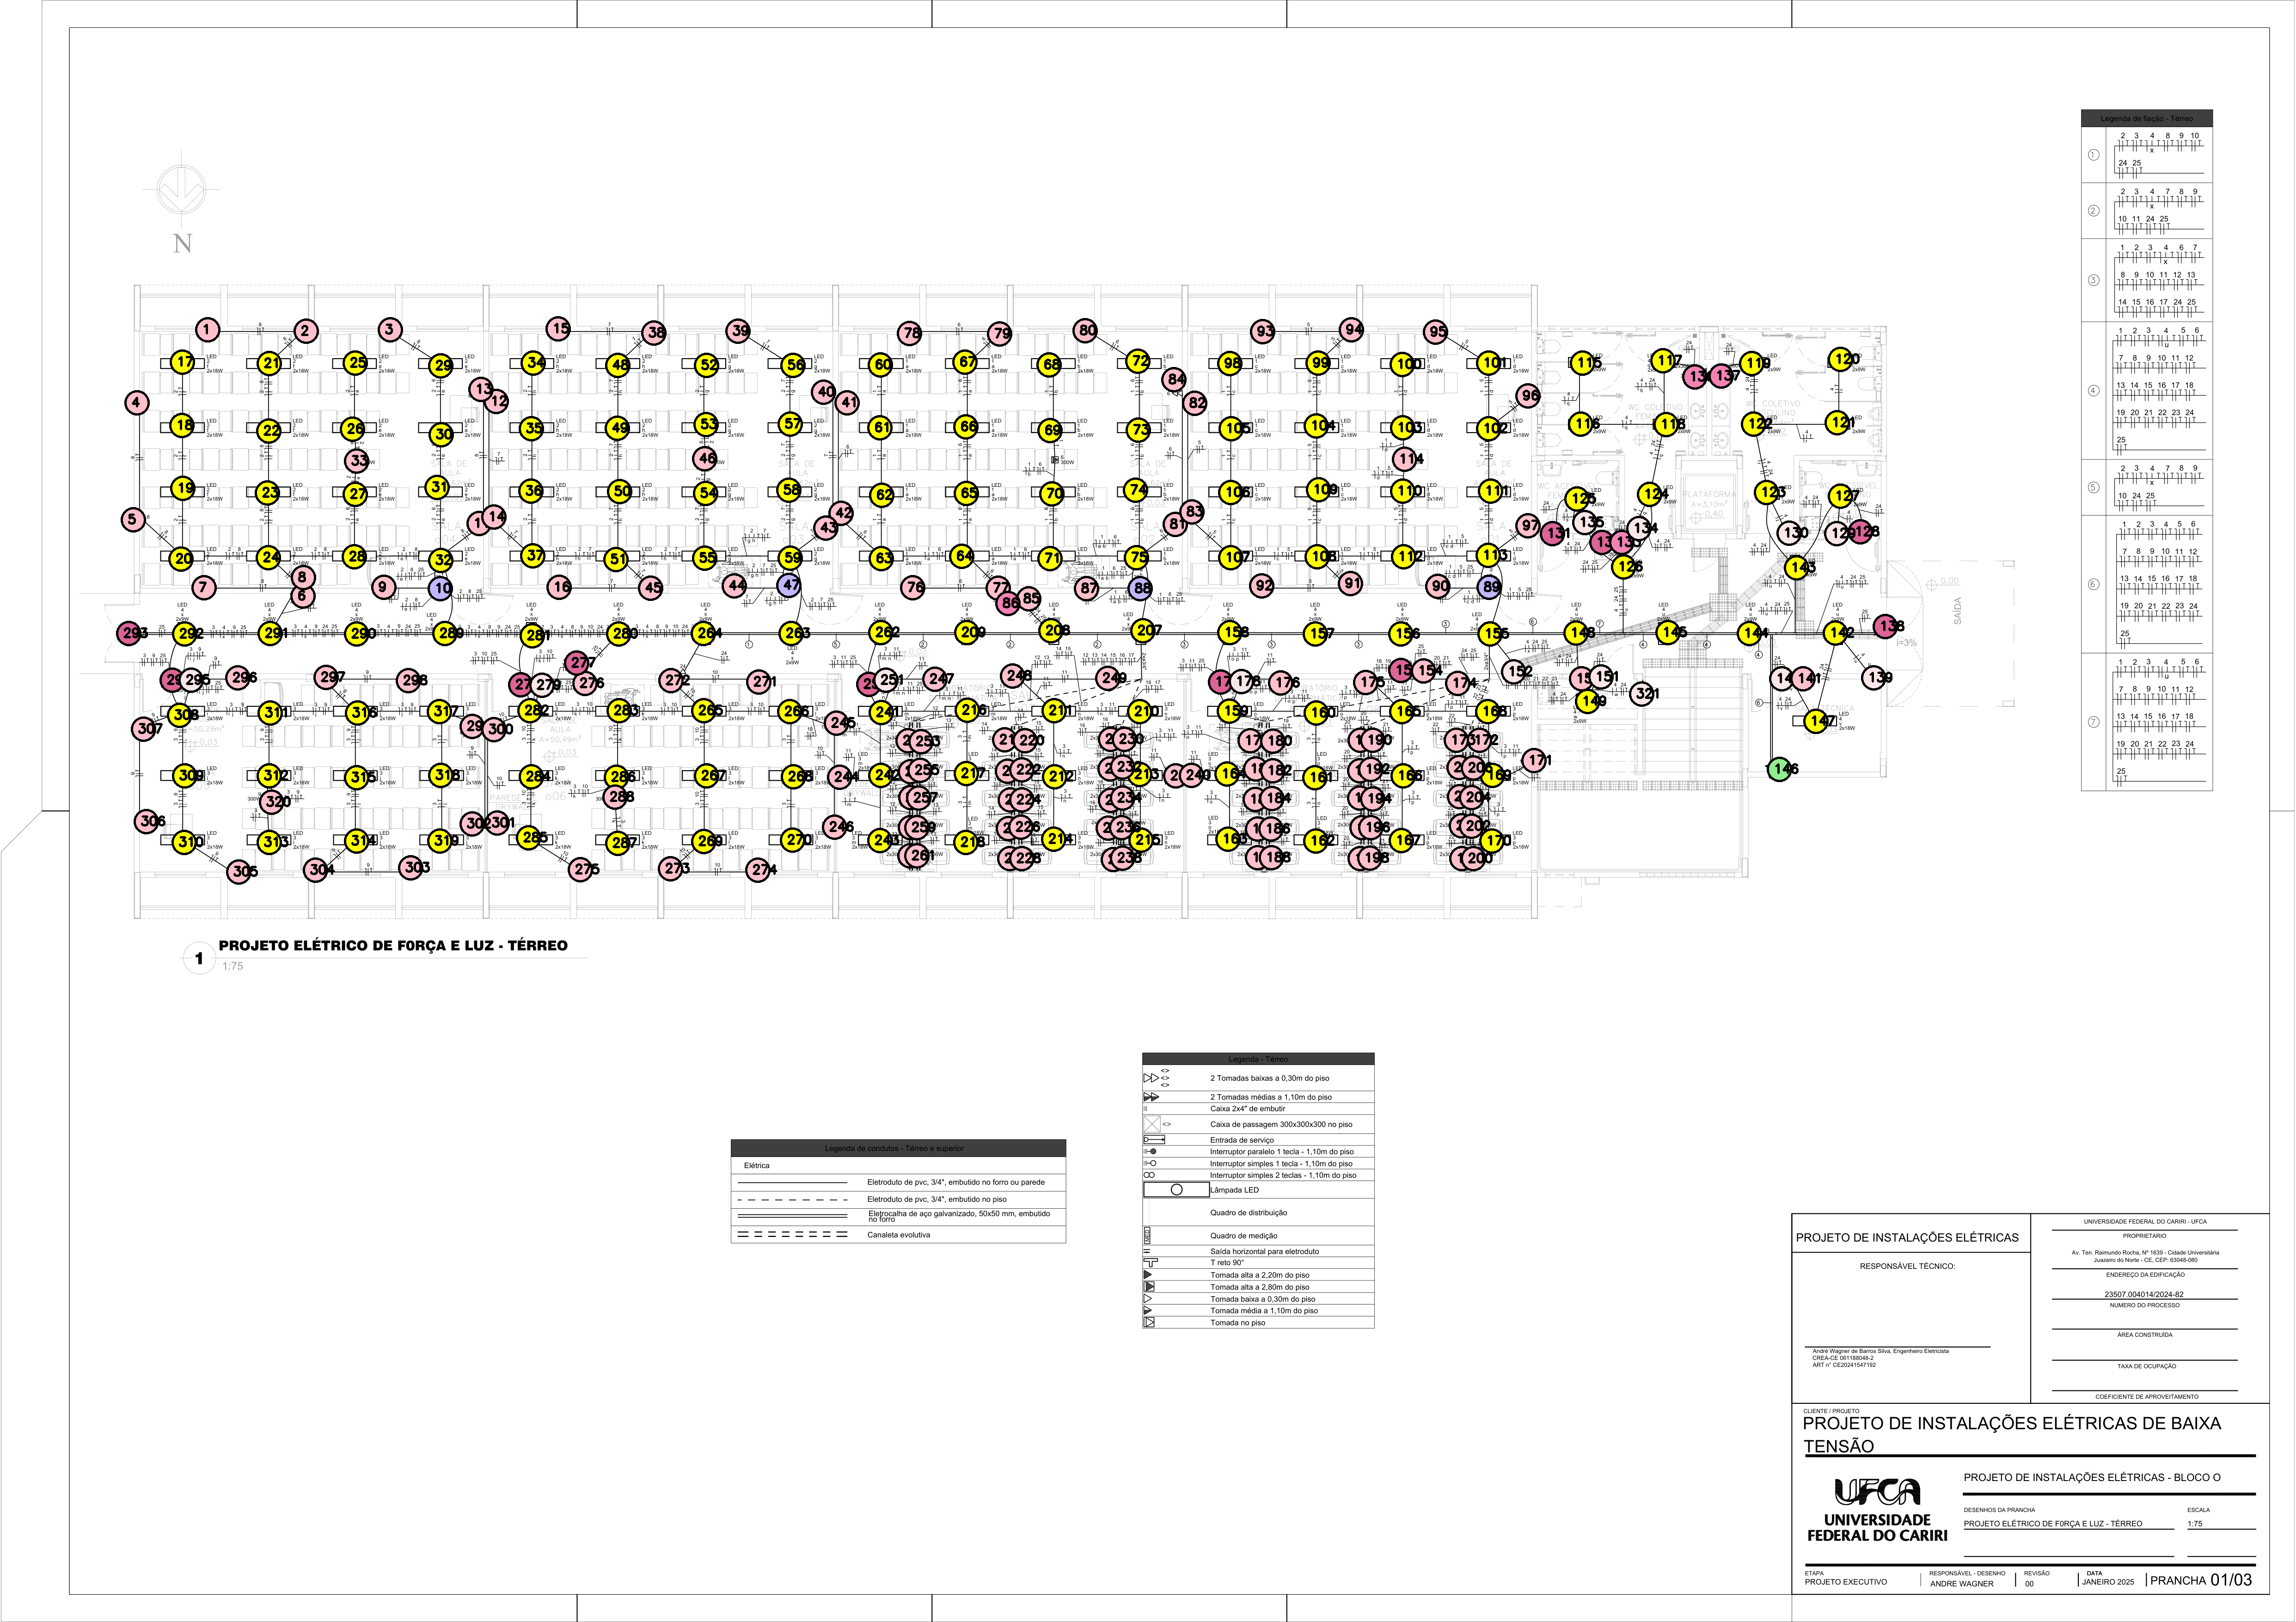
\includegraphics[width=0.95\textwidth]{pagina_1_marcado.png}
\end{figure}

\pagebreak

\subsection{Planta Página 2 - Superior}
\begin{figure}[h!]
\centering
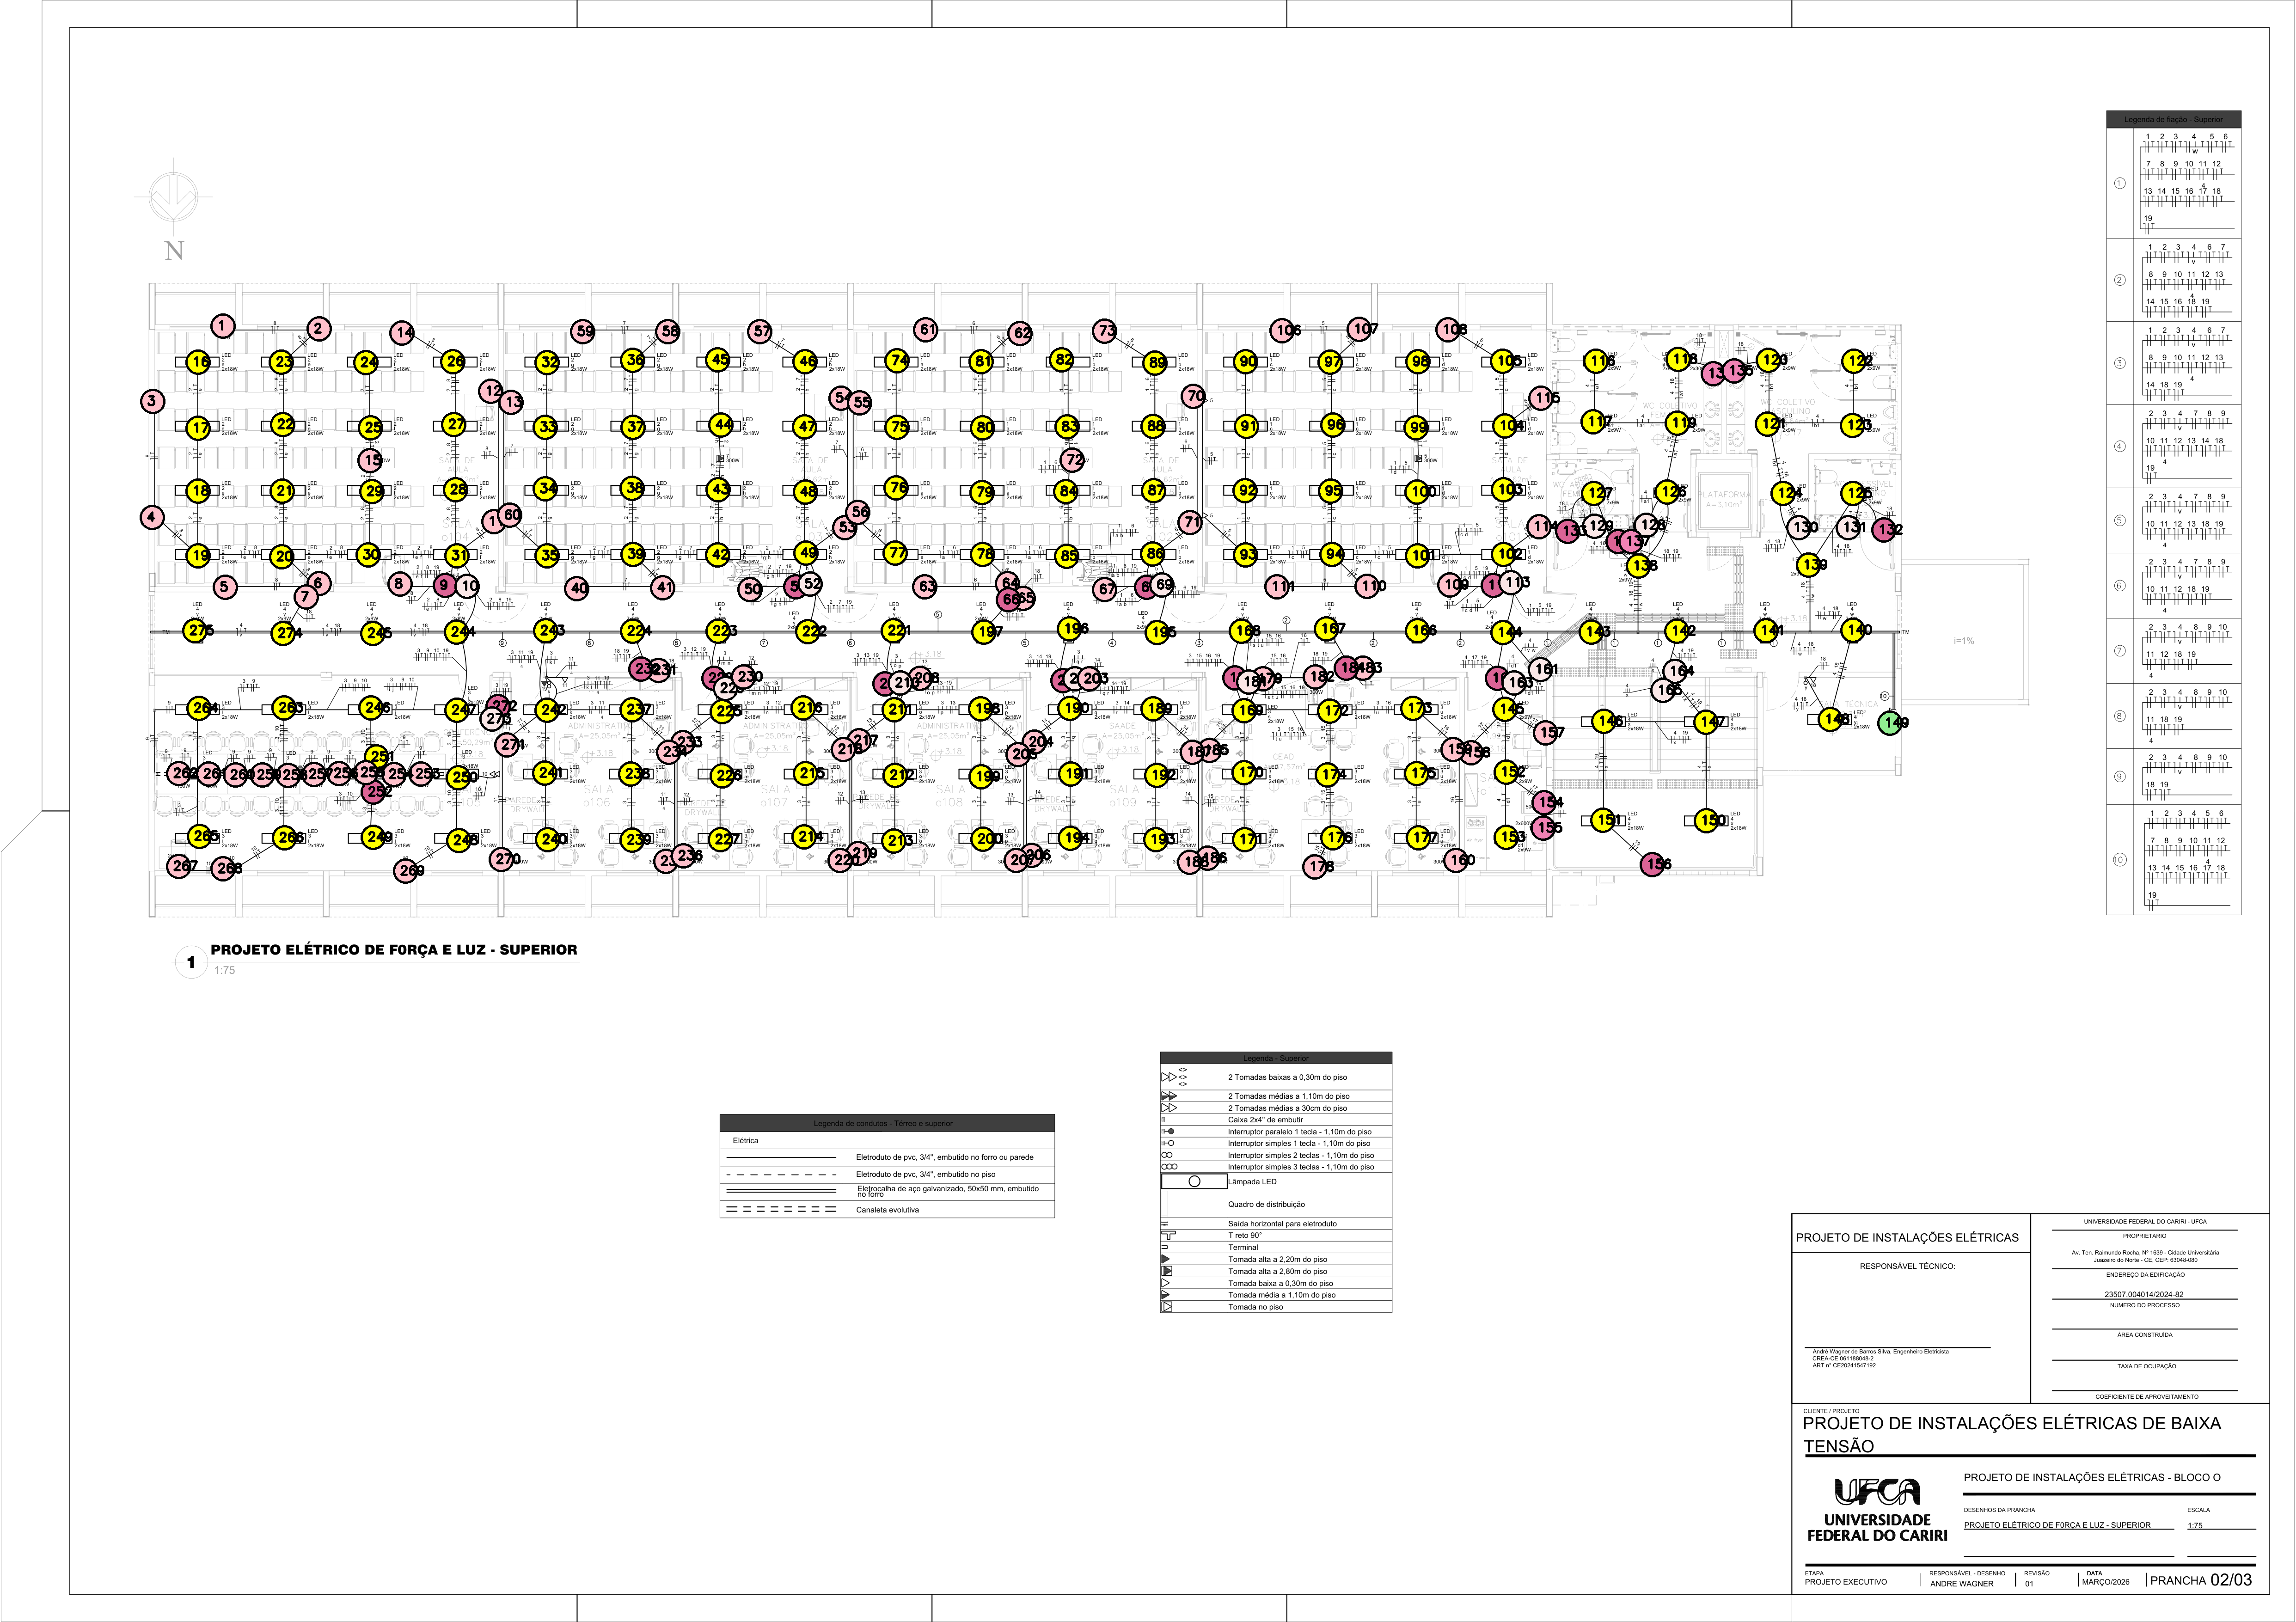
\includegraphics[width=0.95\textwidth]{pagina_2_marcado.png}
\end{figure}

\pagebreak

\subsection{Planta Página 4 - SPDA}
\begin{figure}[h!]
\centering
includegraphics[width=0.95\textwidth]{pagina_4_marcado.png}
\end{figure}

\pagebreak

\subsection{Planta Página 5 - Quadros Térreo}
\begin{figure}[h!]
\centering
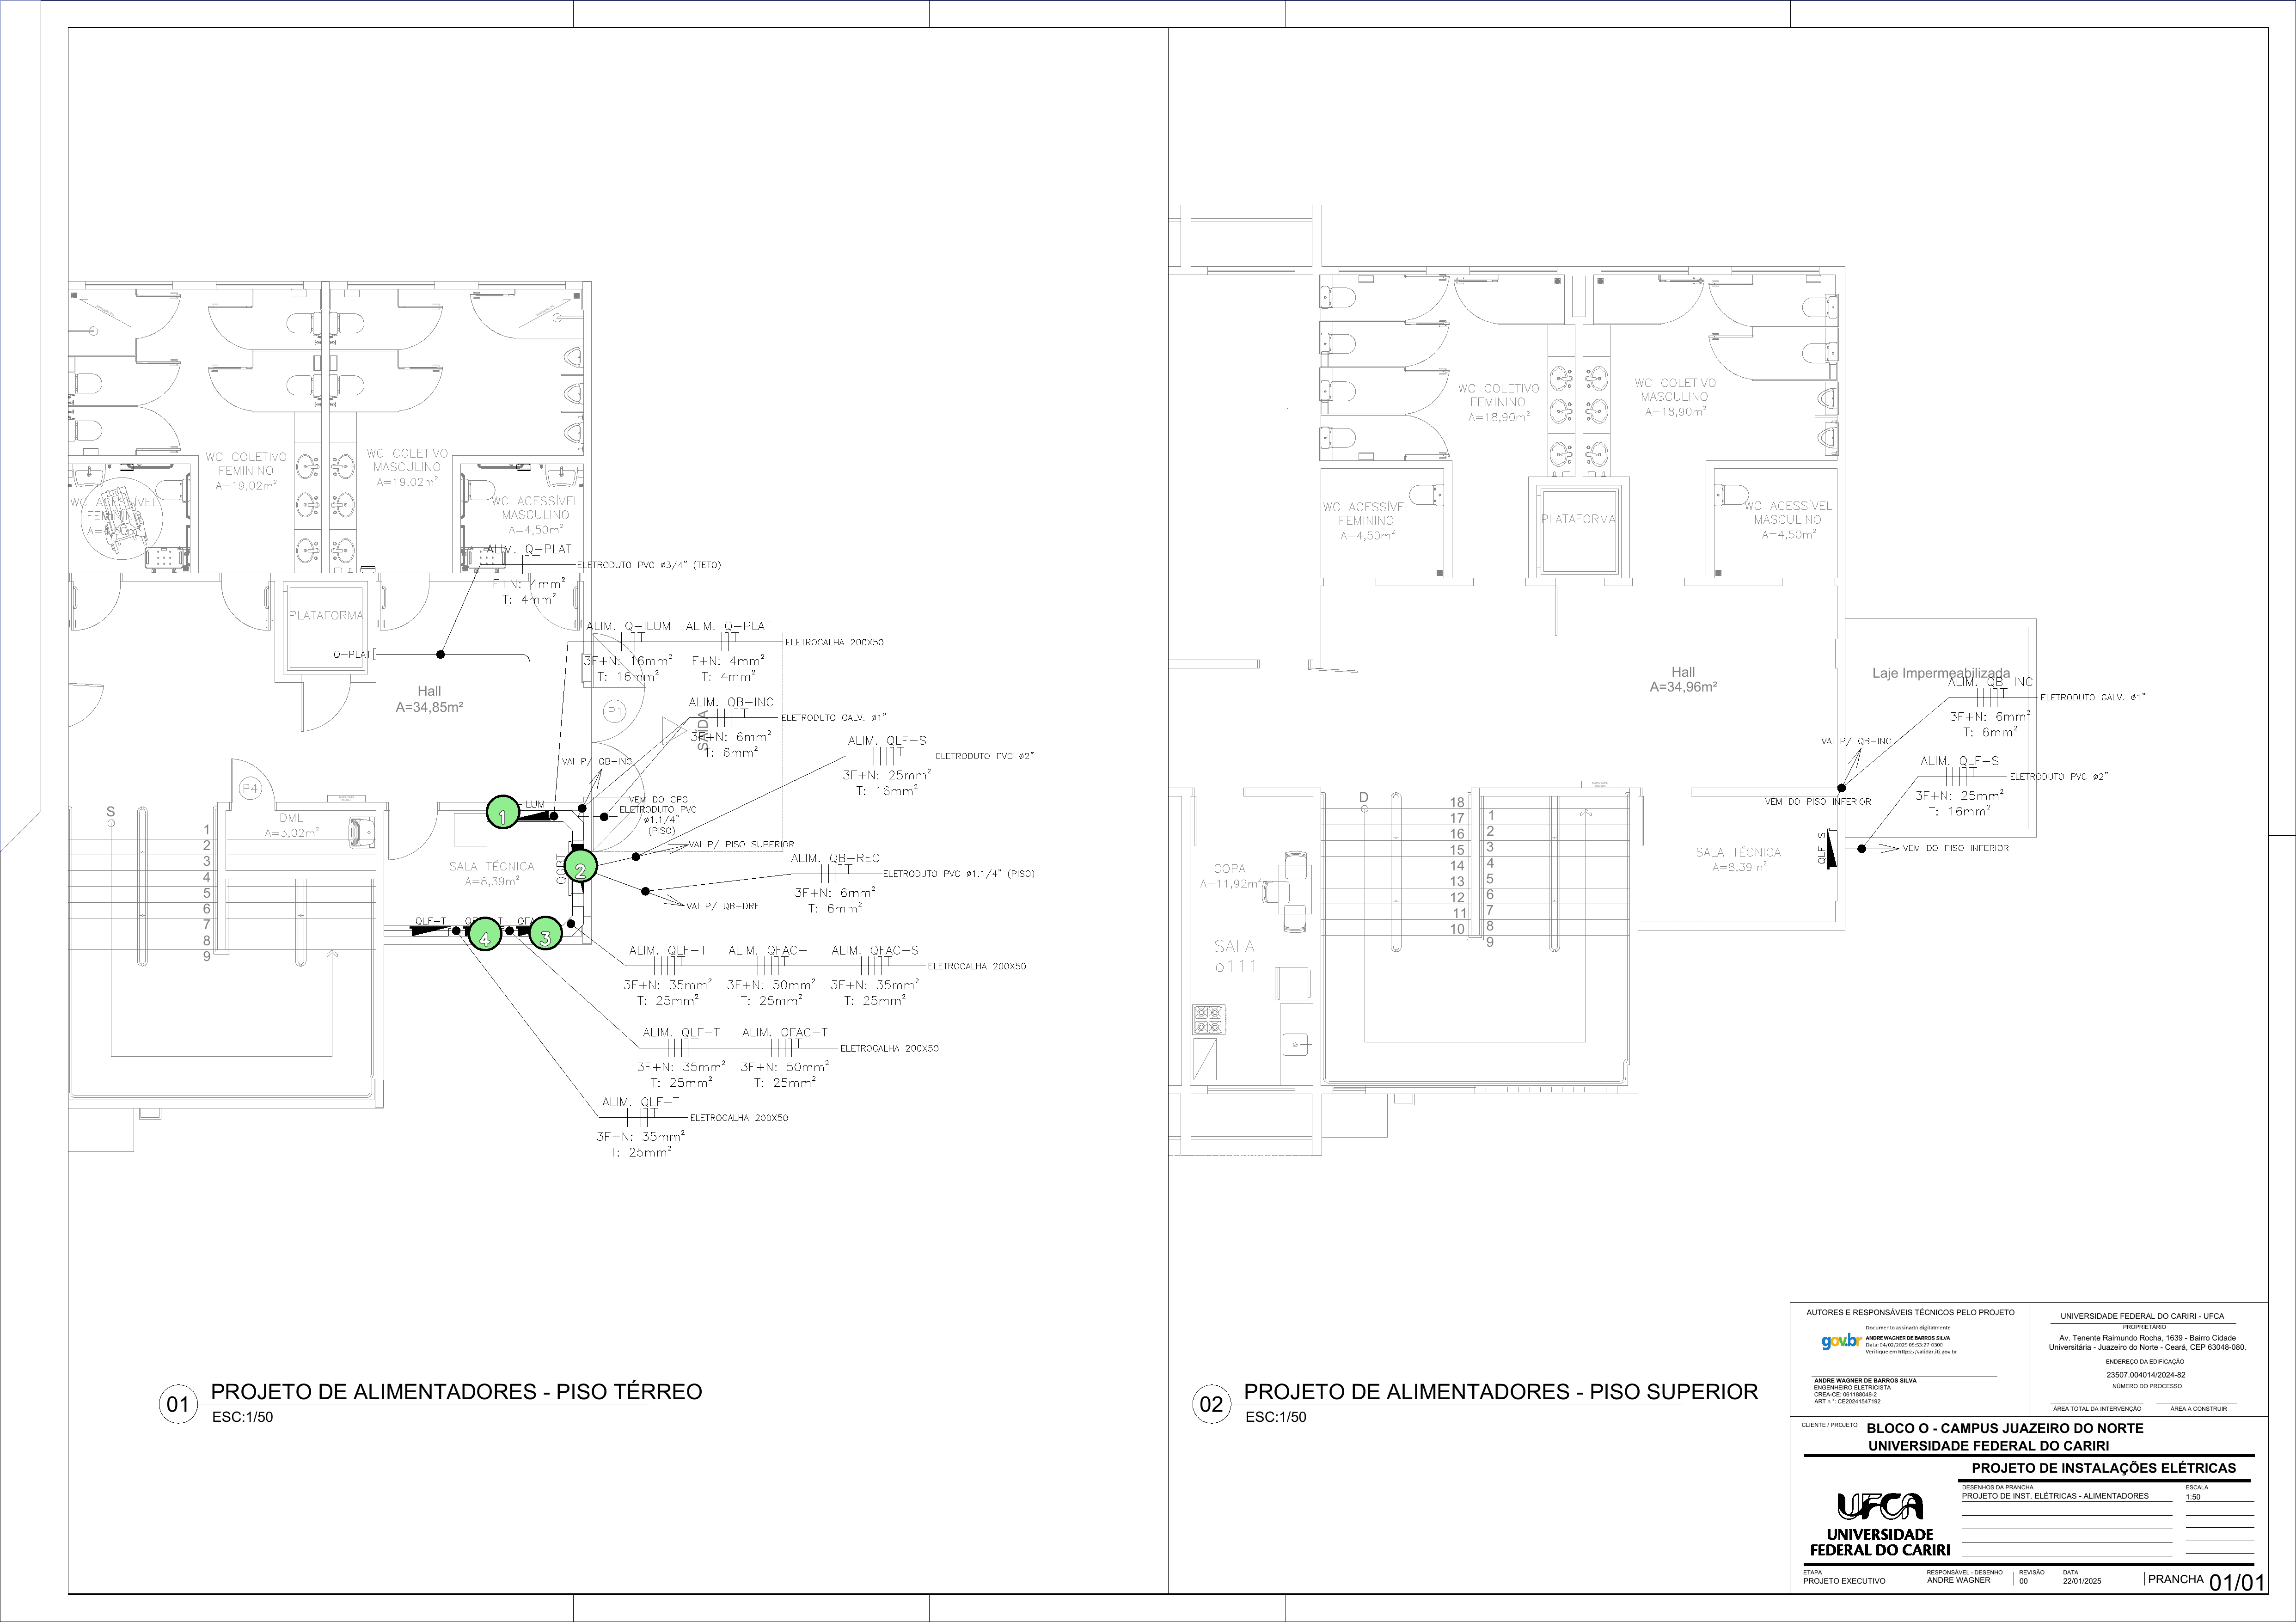
\includegraphics[width=0.95\textwidth]{pagina_5_marcado.png}
\end{figure}

\pagebreak

\subsection{Planta Página 6 - Quadros Superior}
\begin{figure}[h!]
\centering
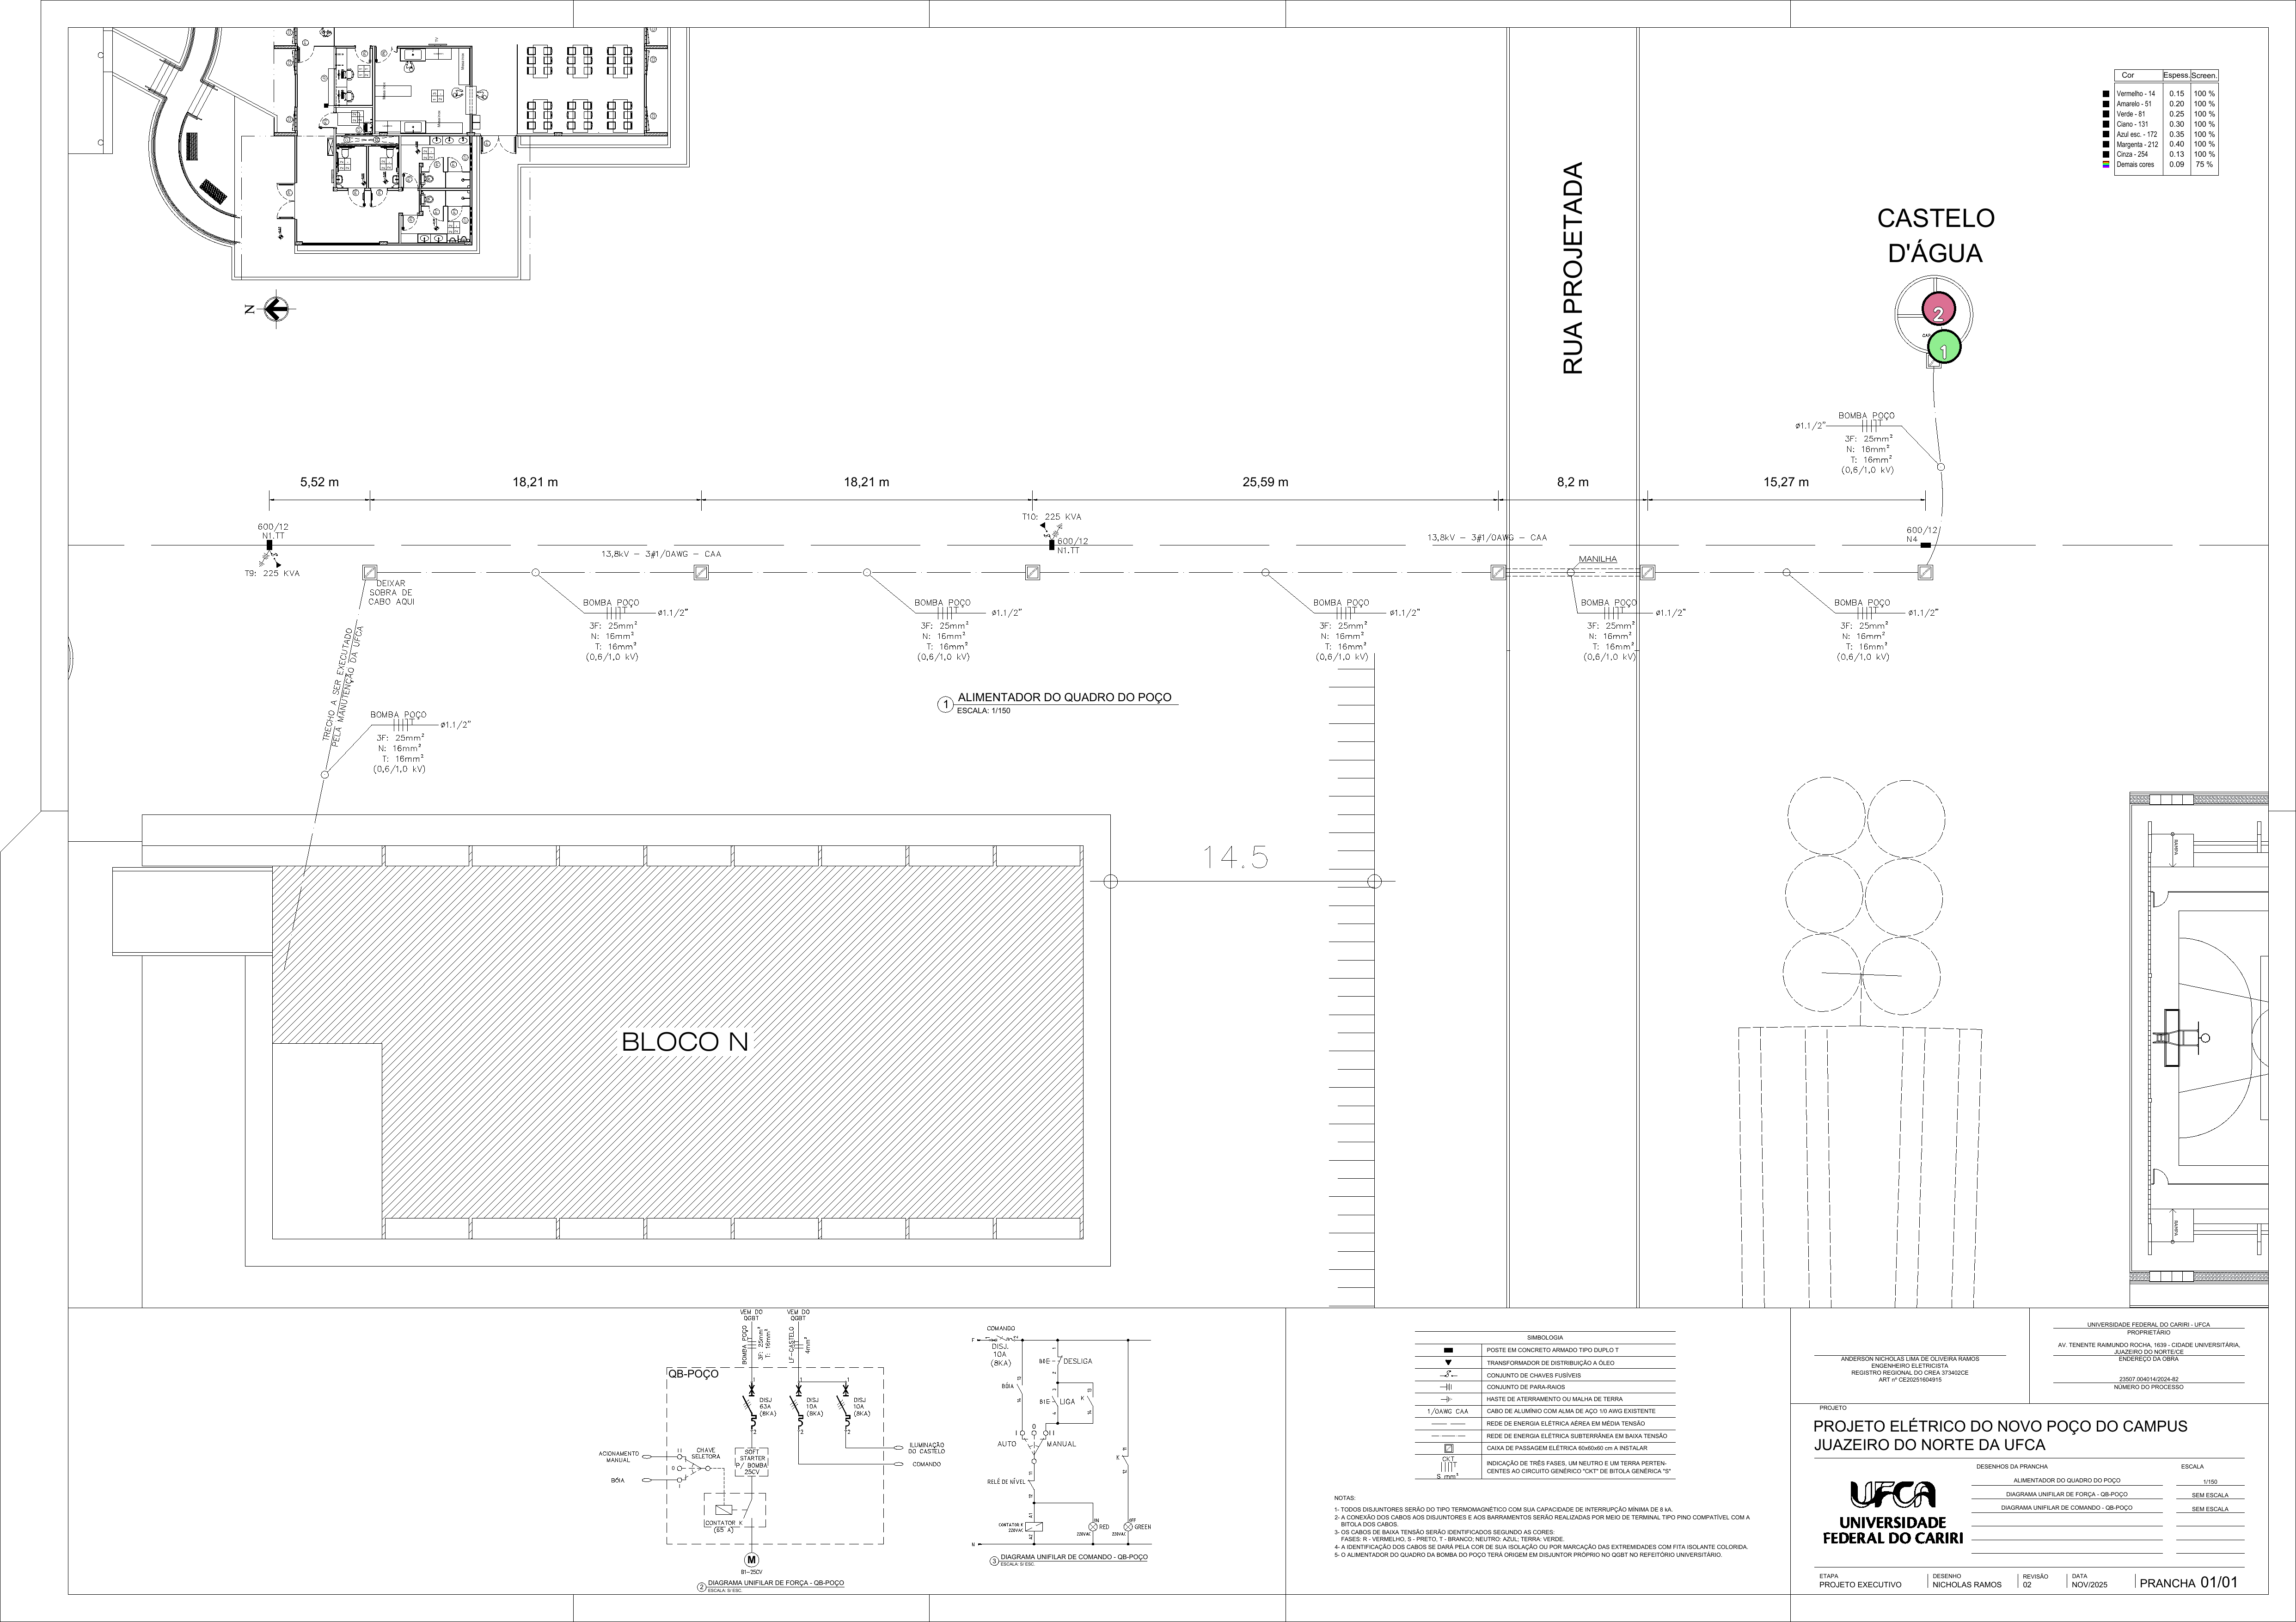
\includegraphics[width=0.95\textwidth]{pagina_6_marcado.png}
\end{figure}

\pagebreak

\subsection{Planta Página 8 - Bombas}
\begin{figure}[h!]
\centering
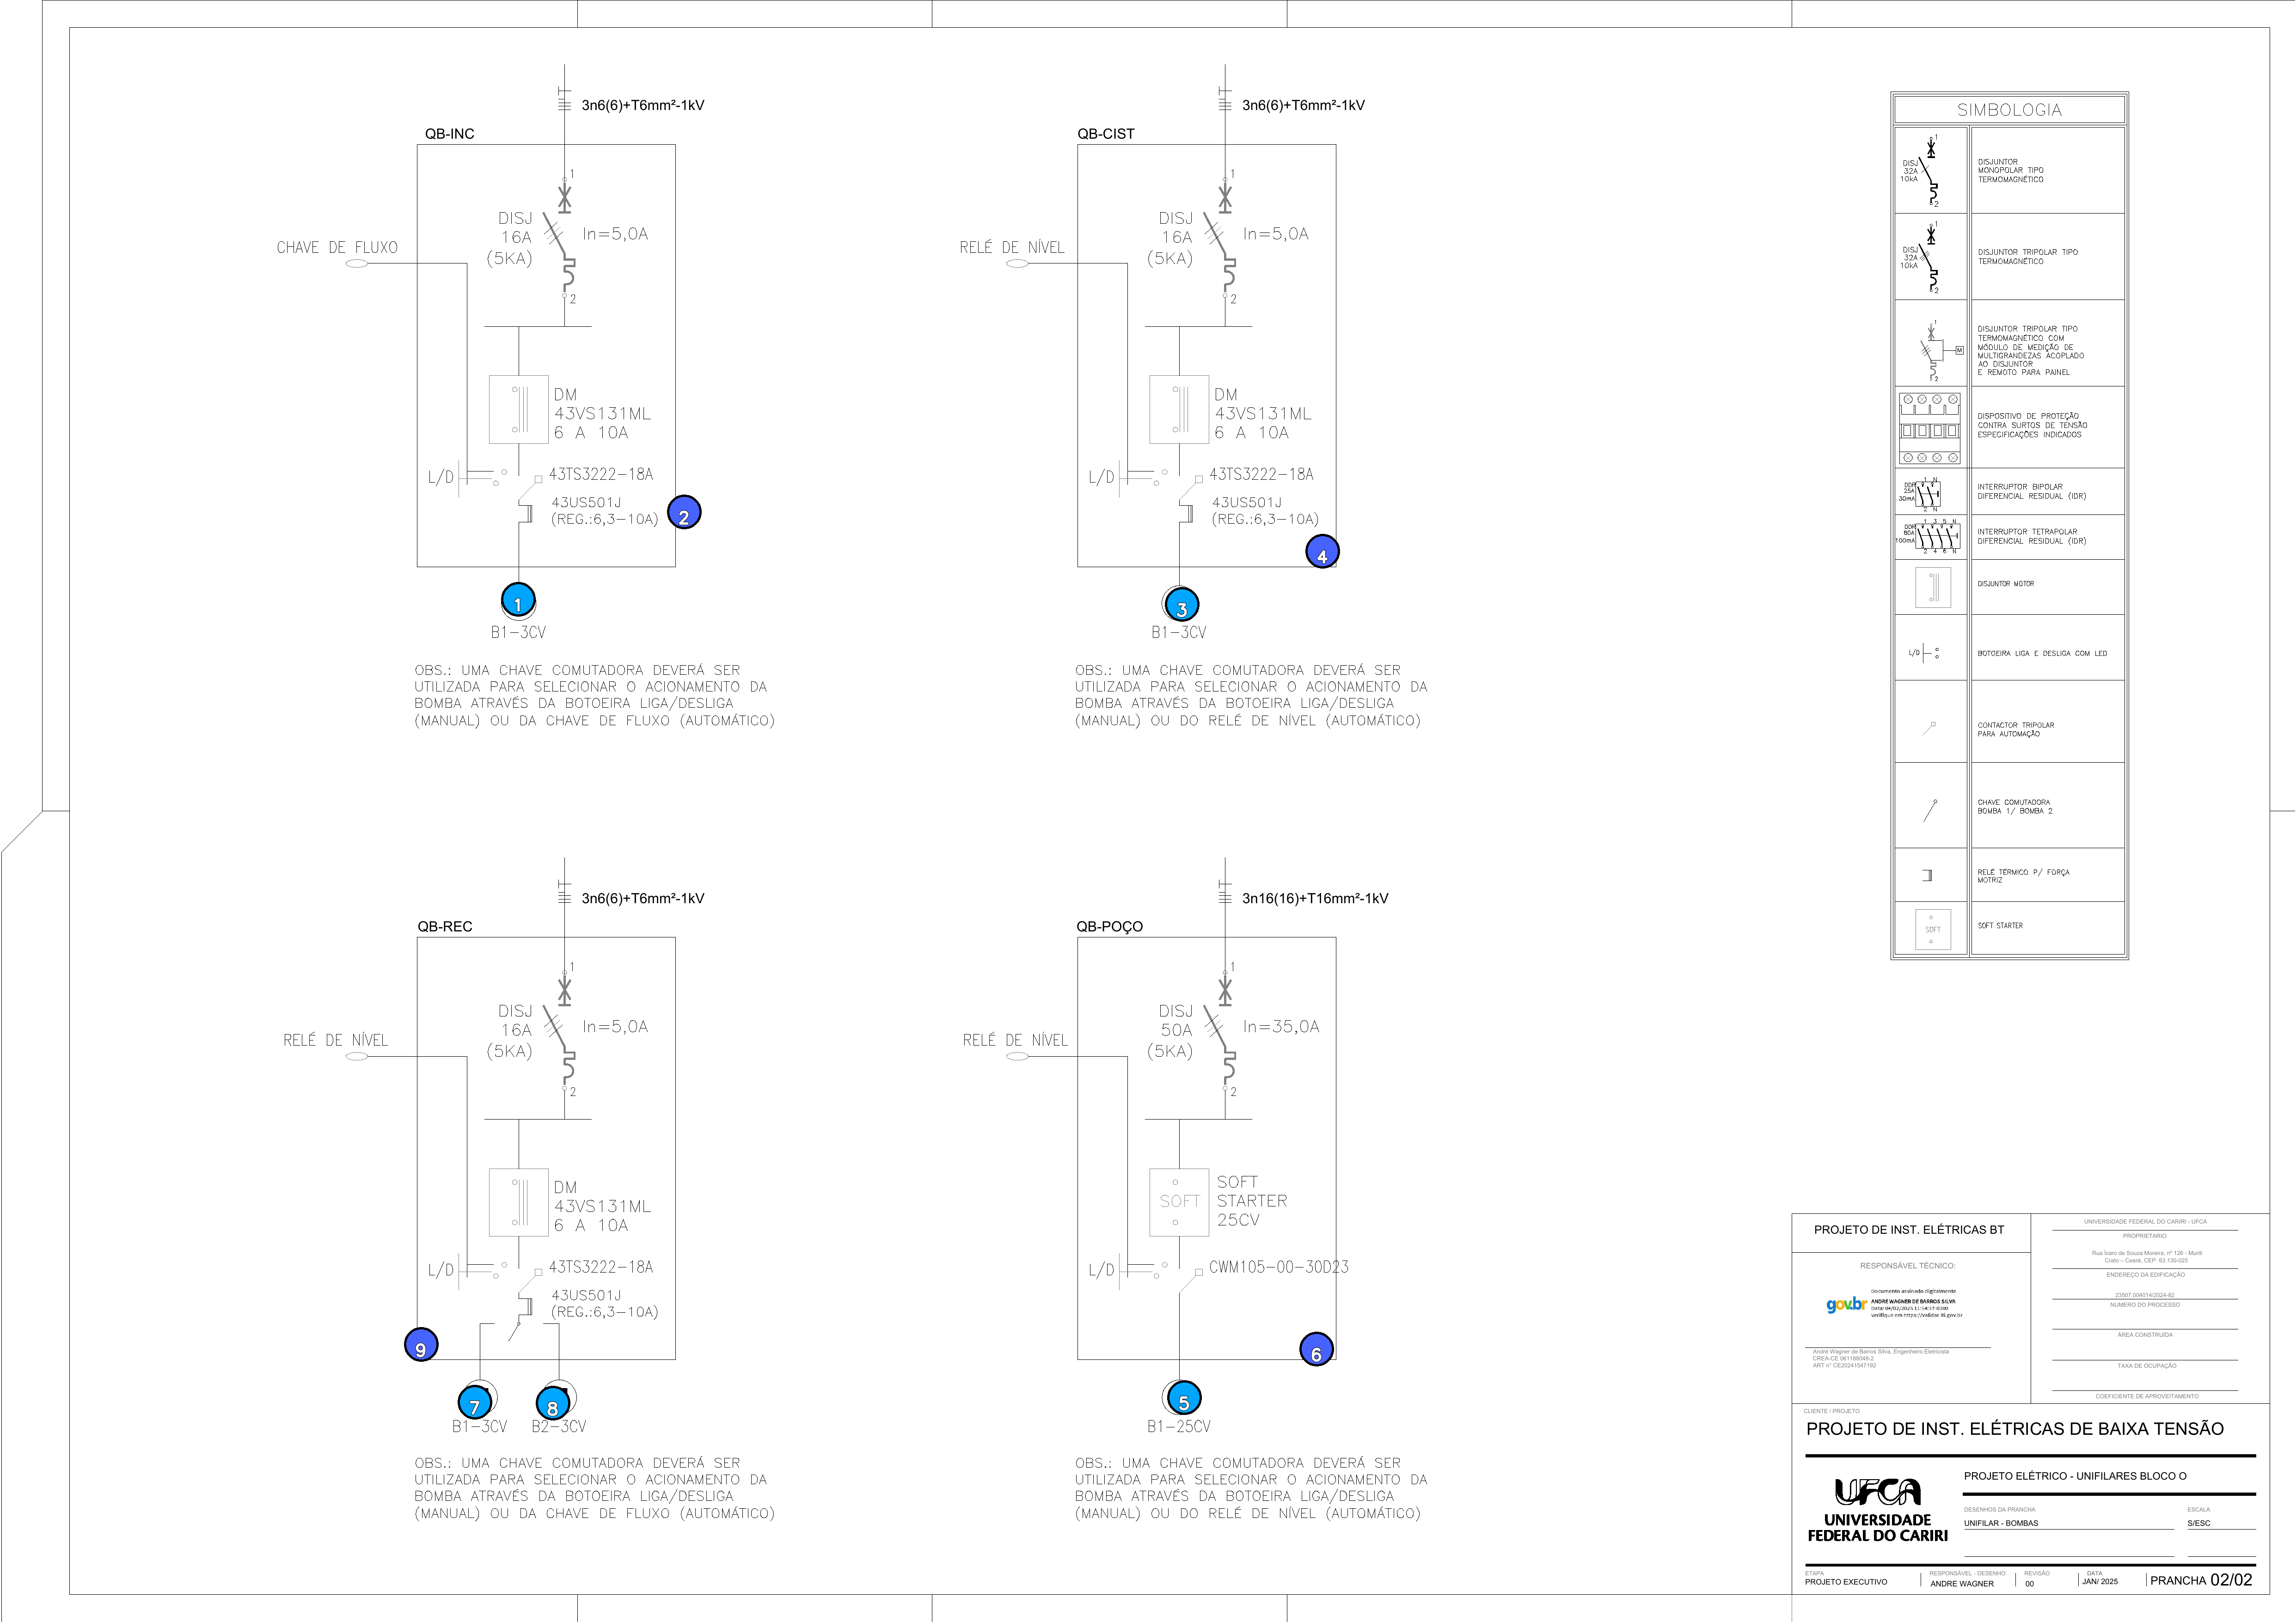
\includegraphics[width=0.95\textwidth]{pagina_8_marcado.png}
\end{figure}

\pagebreak

\subsection{Planta Página 9 - RTA}
\begin{figure}[h!]
\centering
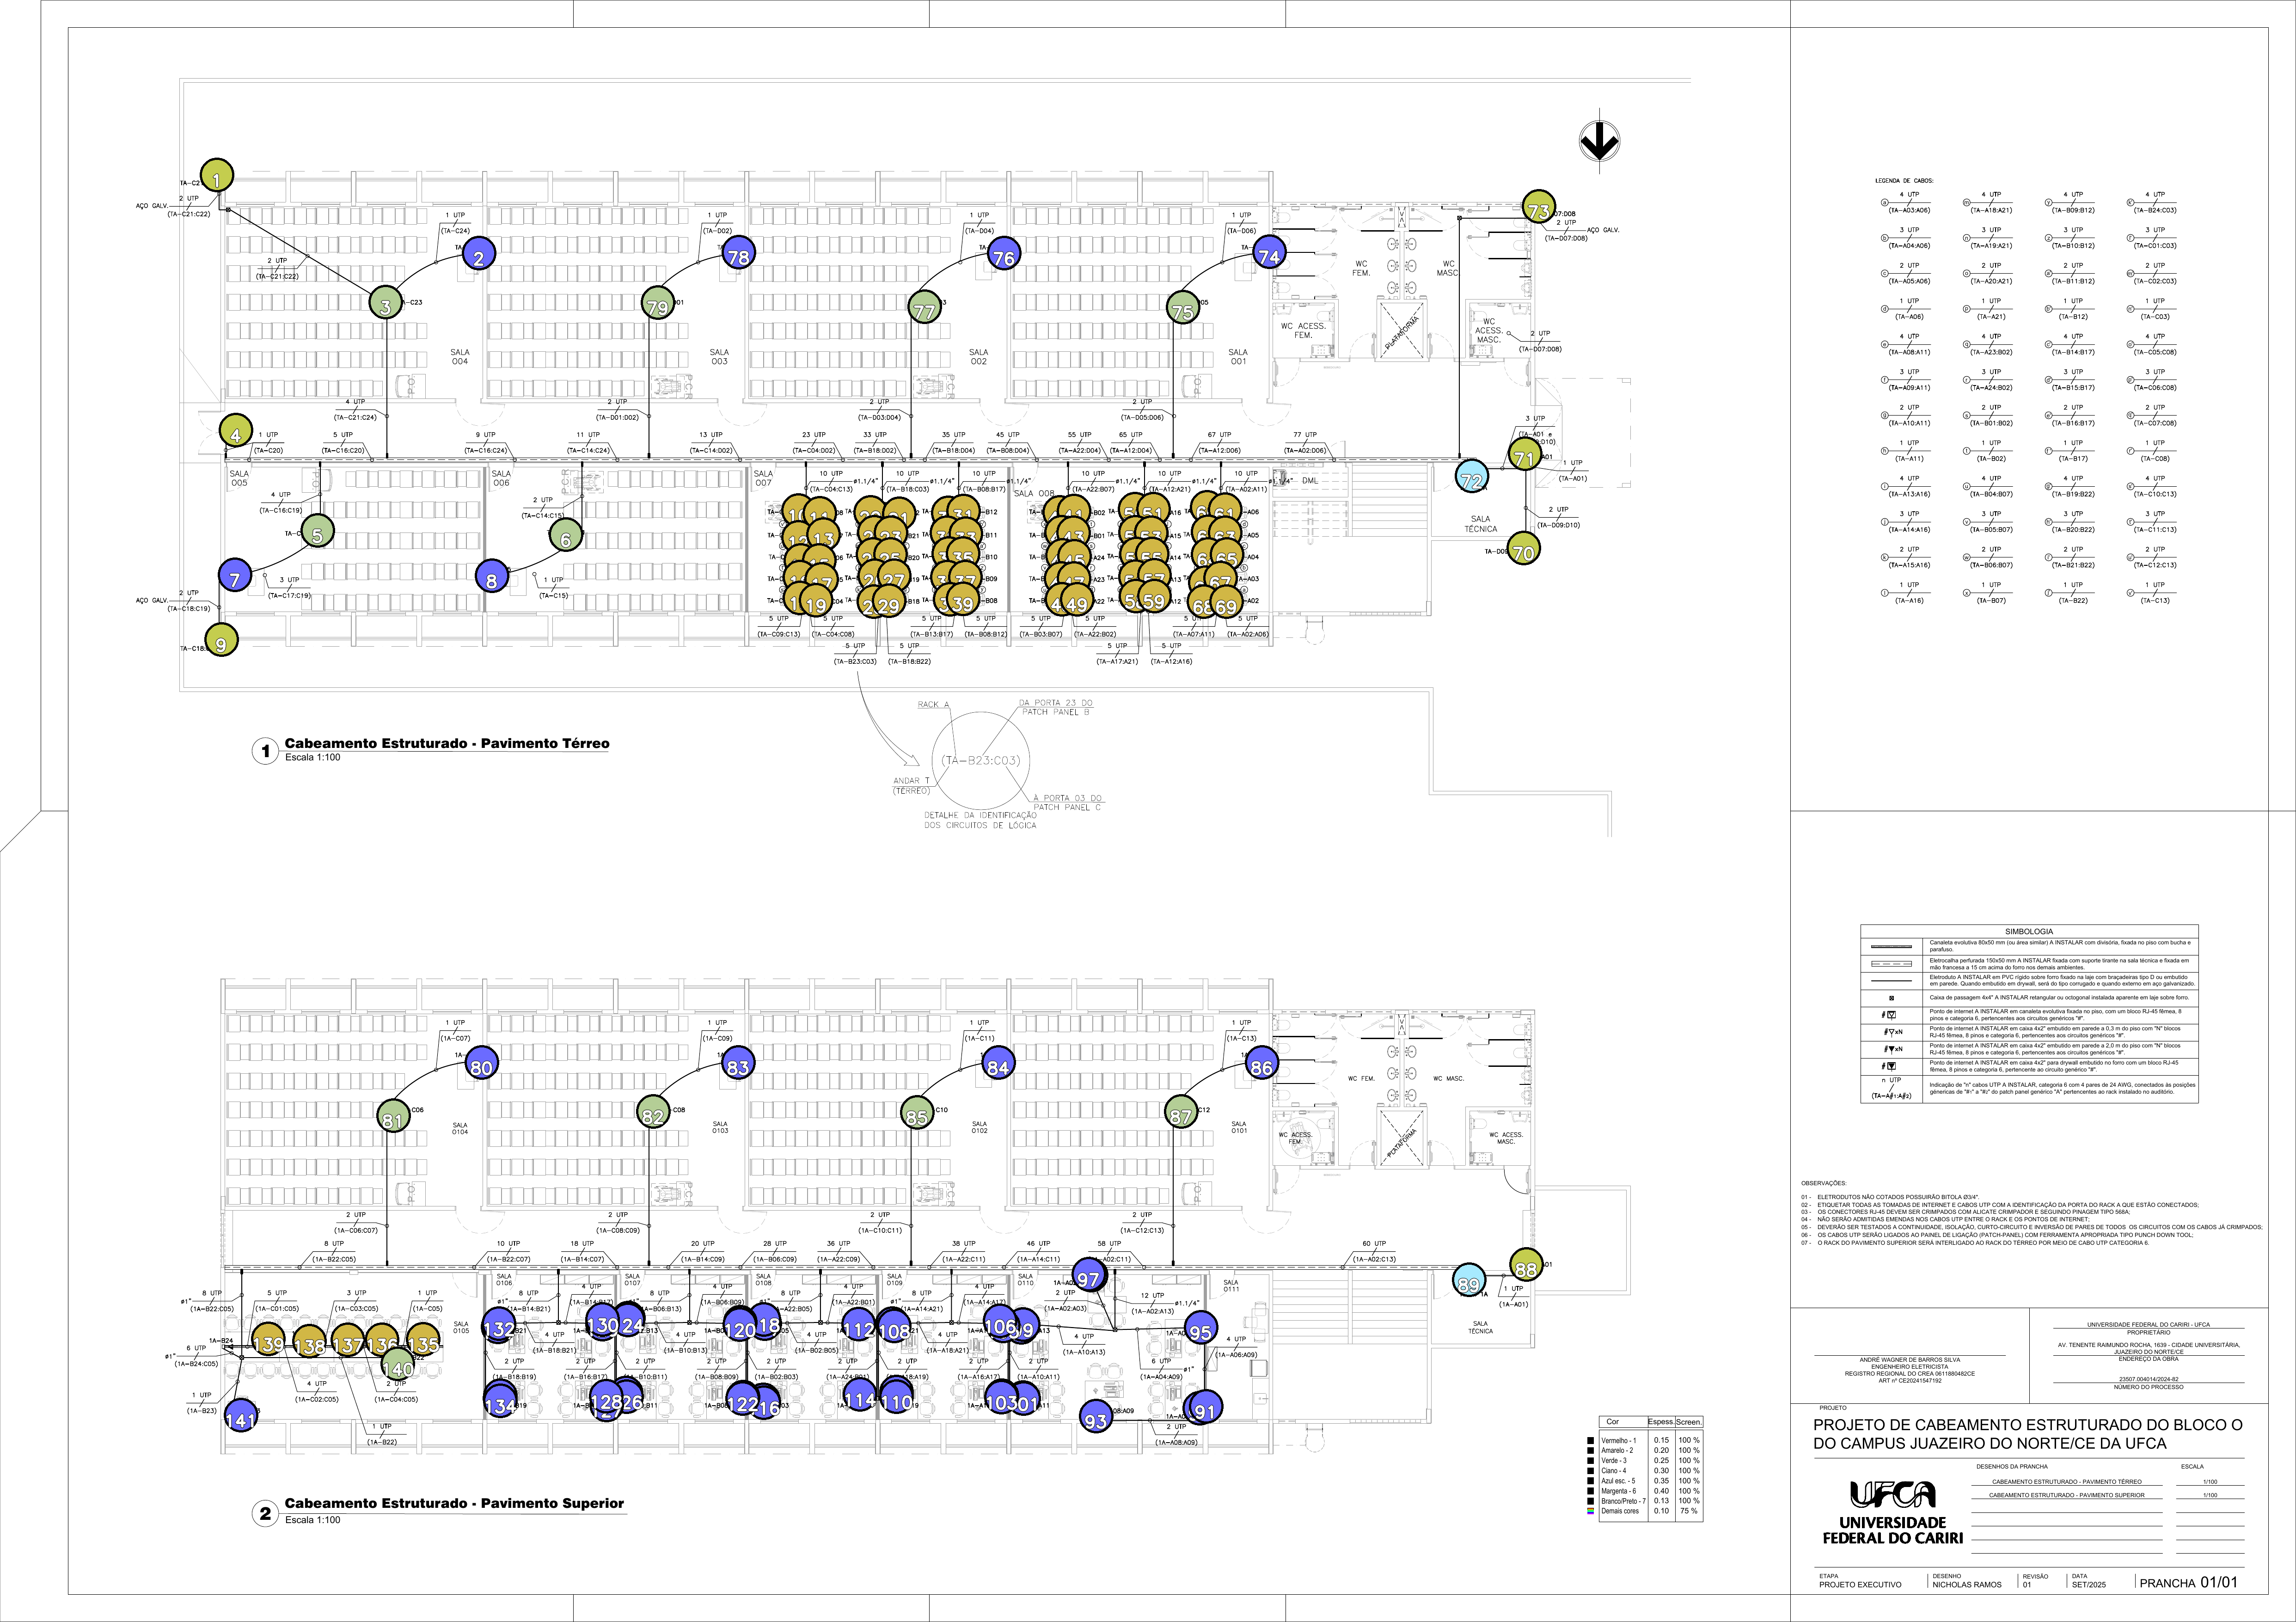
\includegraphics[width=0.95\textwidth]{pagina_9_marcado.png}
\end{figure}

\pagebreak

\subsection{Planta Página 10 - Iluminação Externa 1}
\begin{figure}[h!]
\centering
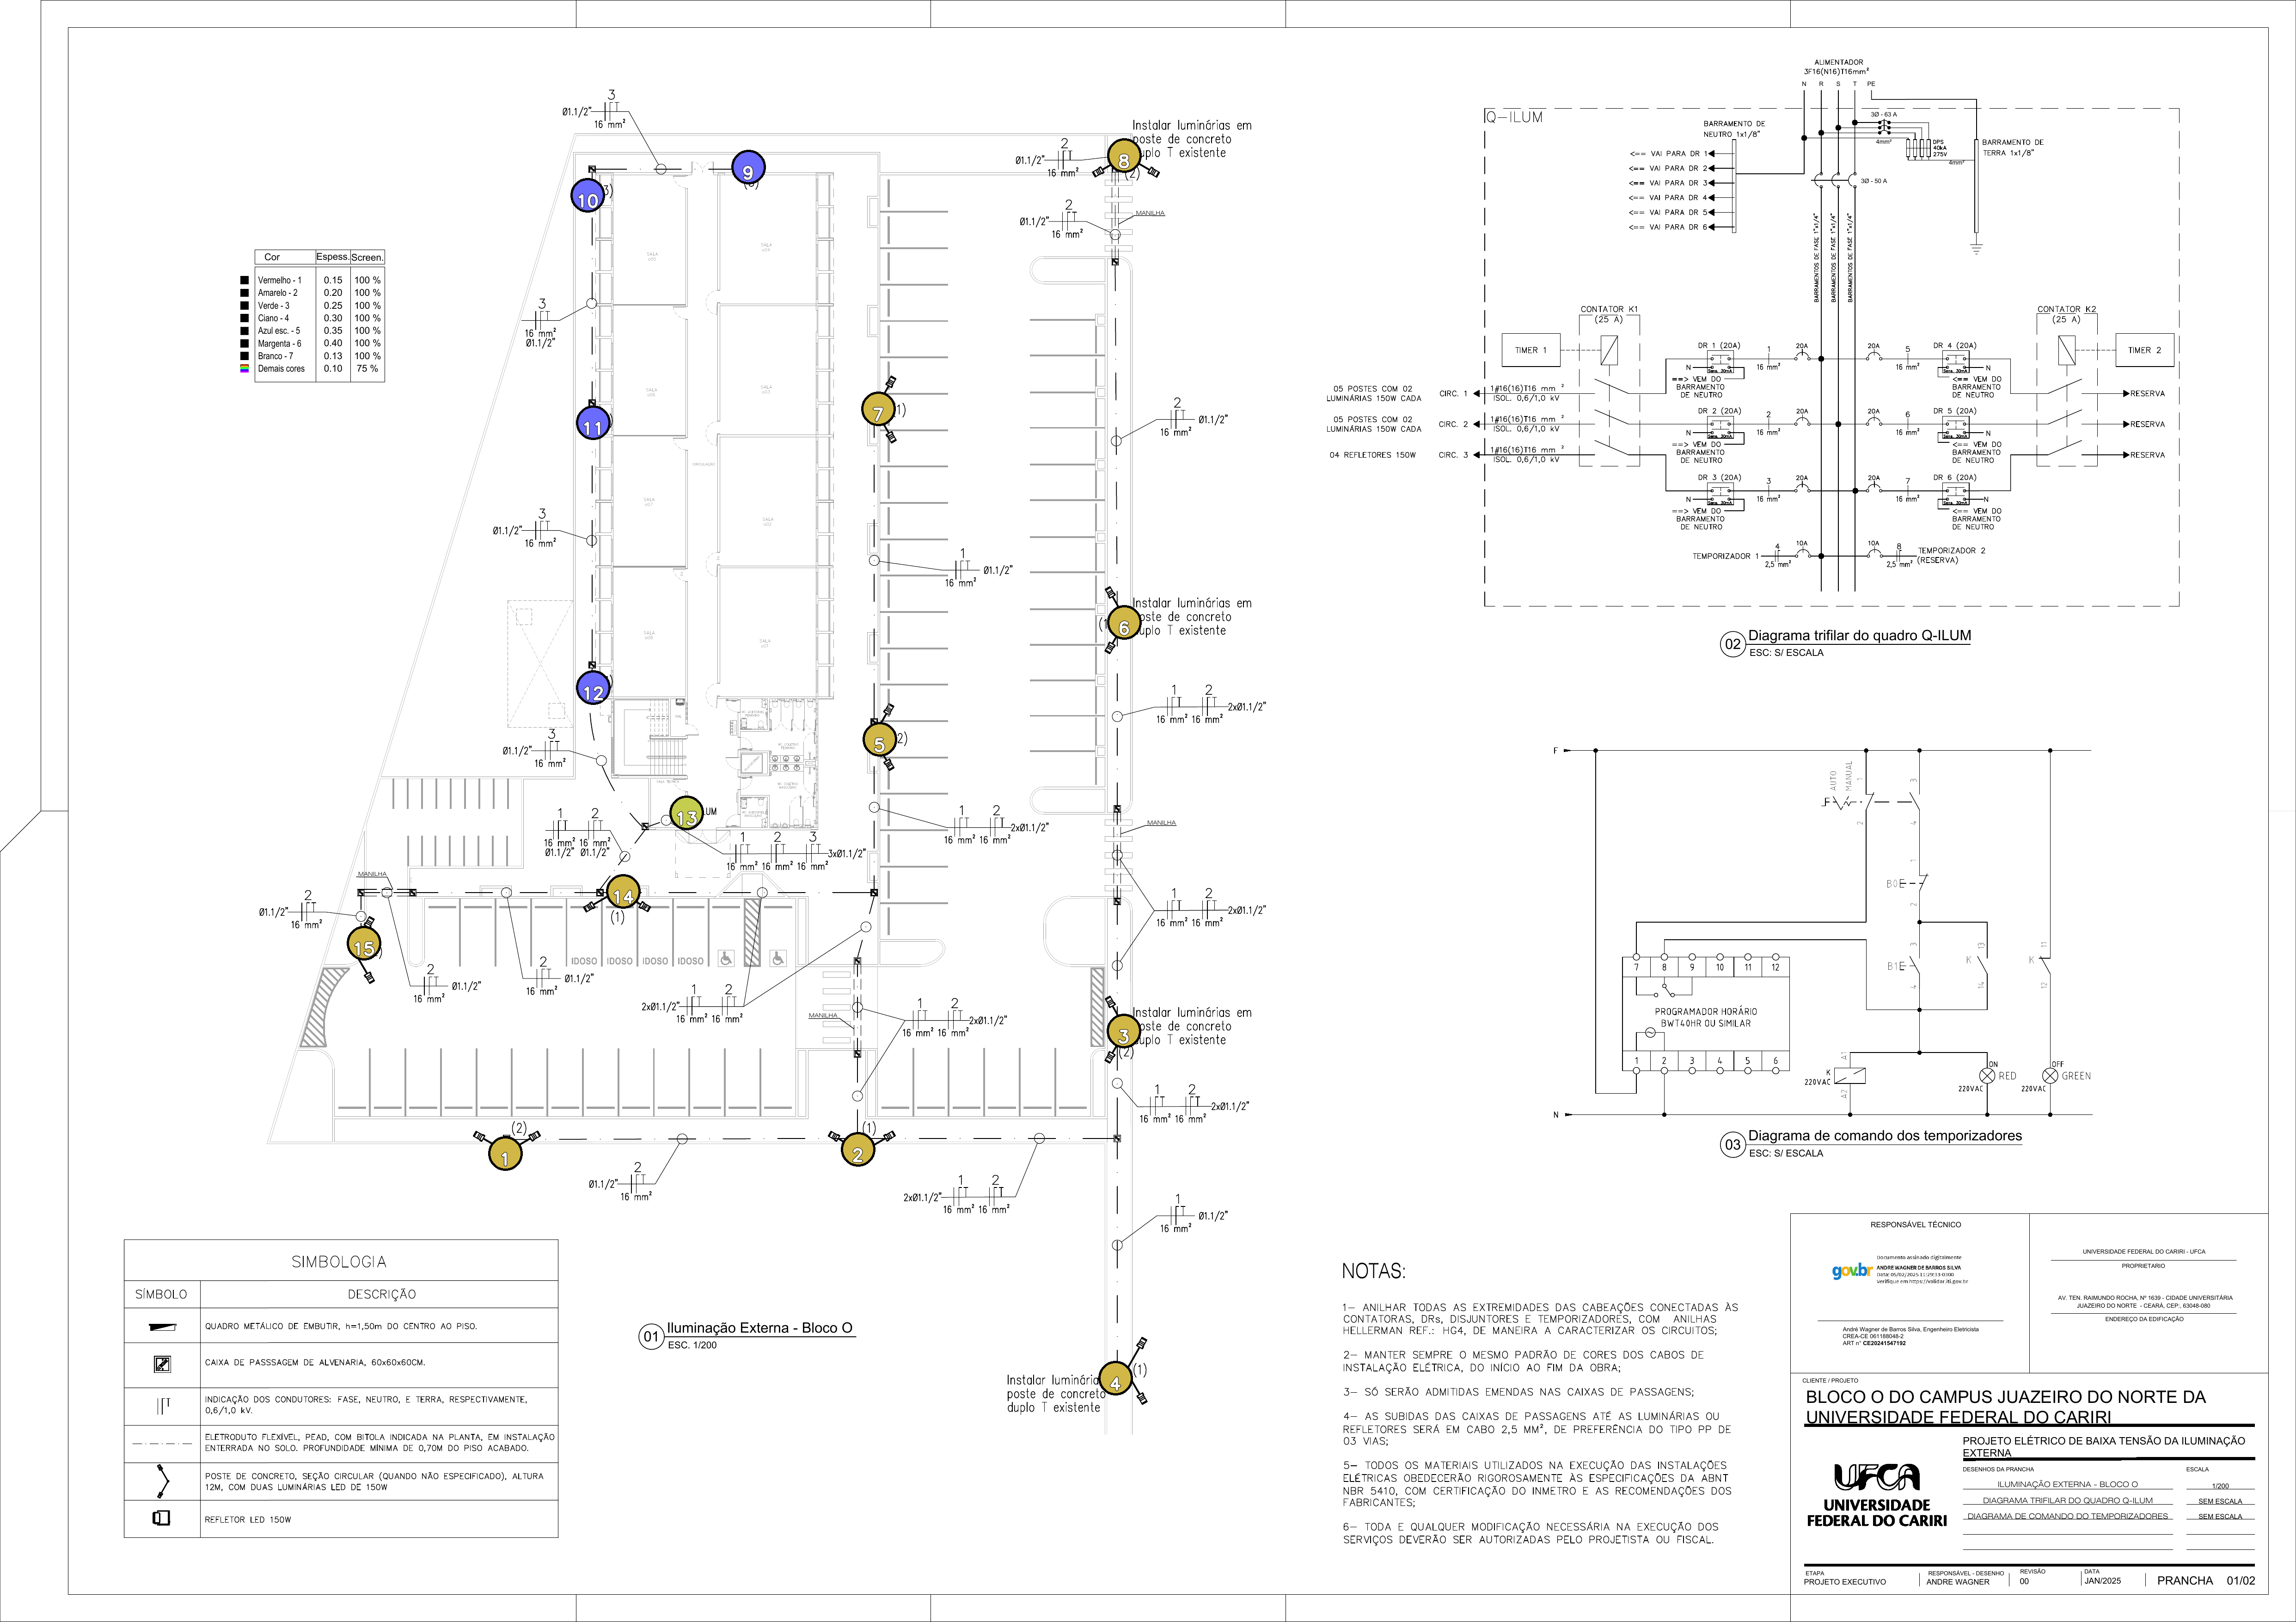
\includegraphics[width=0.95\textwidth]{pagina_10_marcado.png}
\end{figure}

\pagebreak

\subsection{Planta Página 11 - Iluminação Externa 2}
\begin{figure}[h!]
\centering
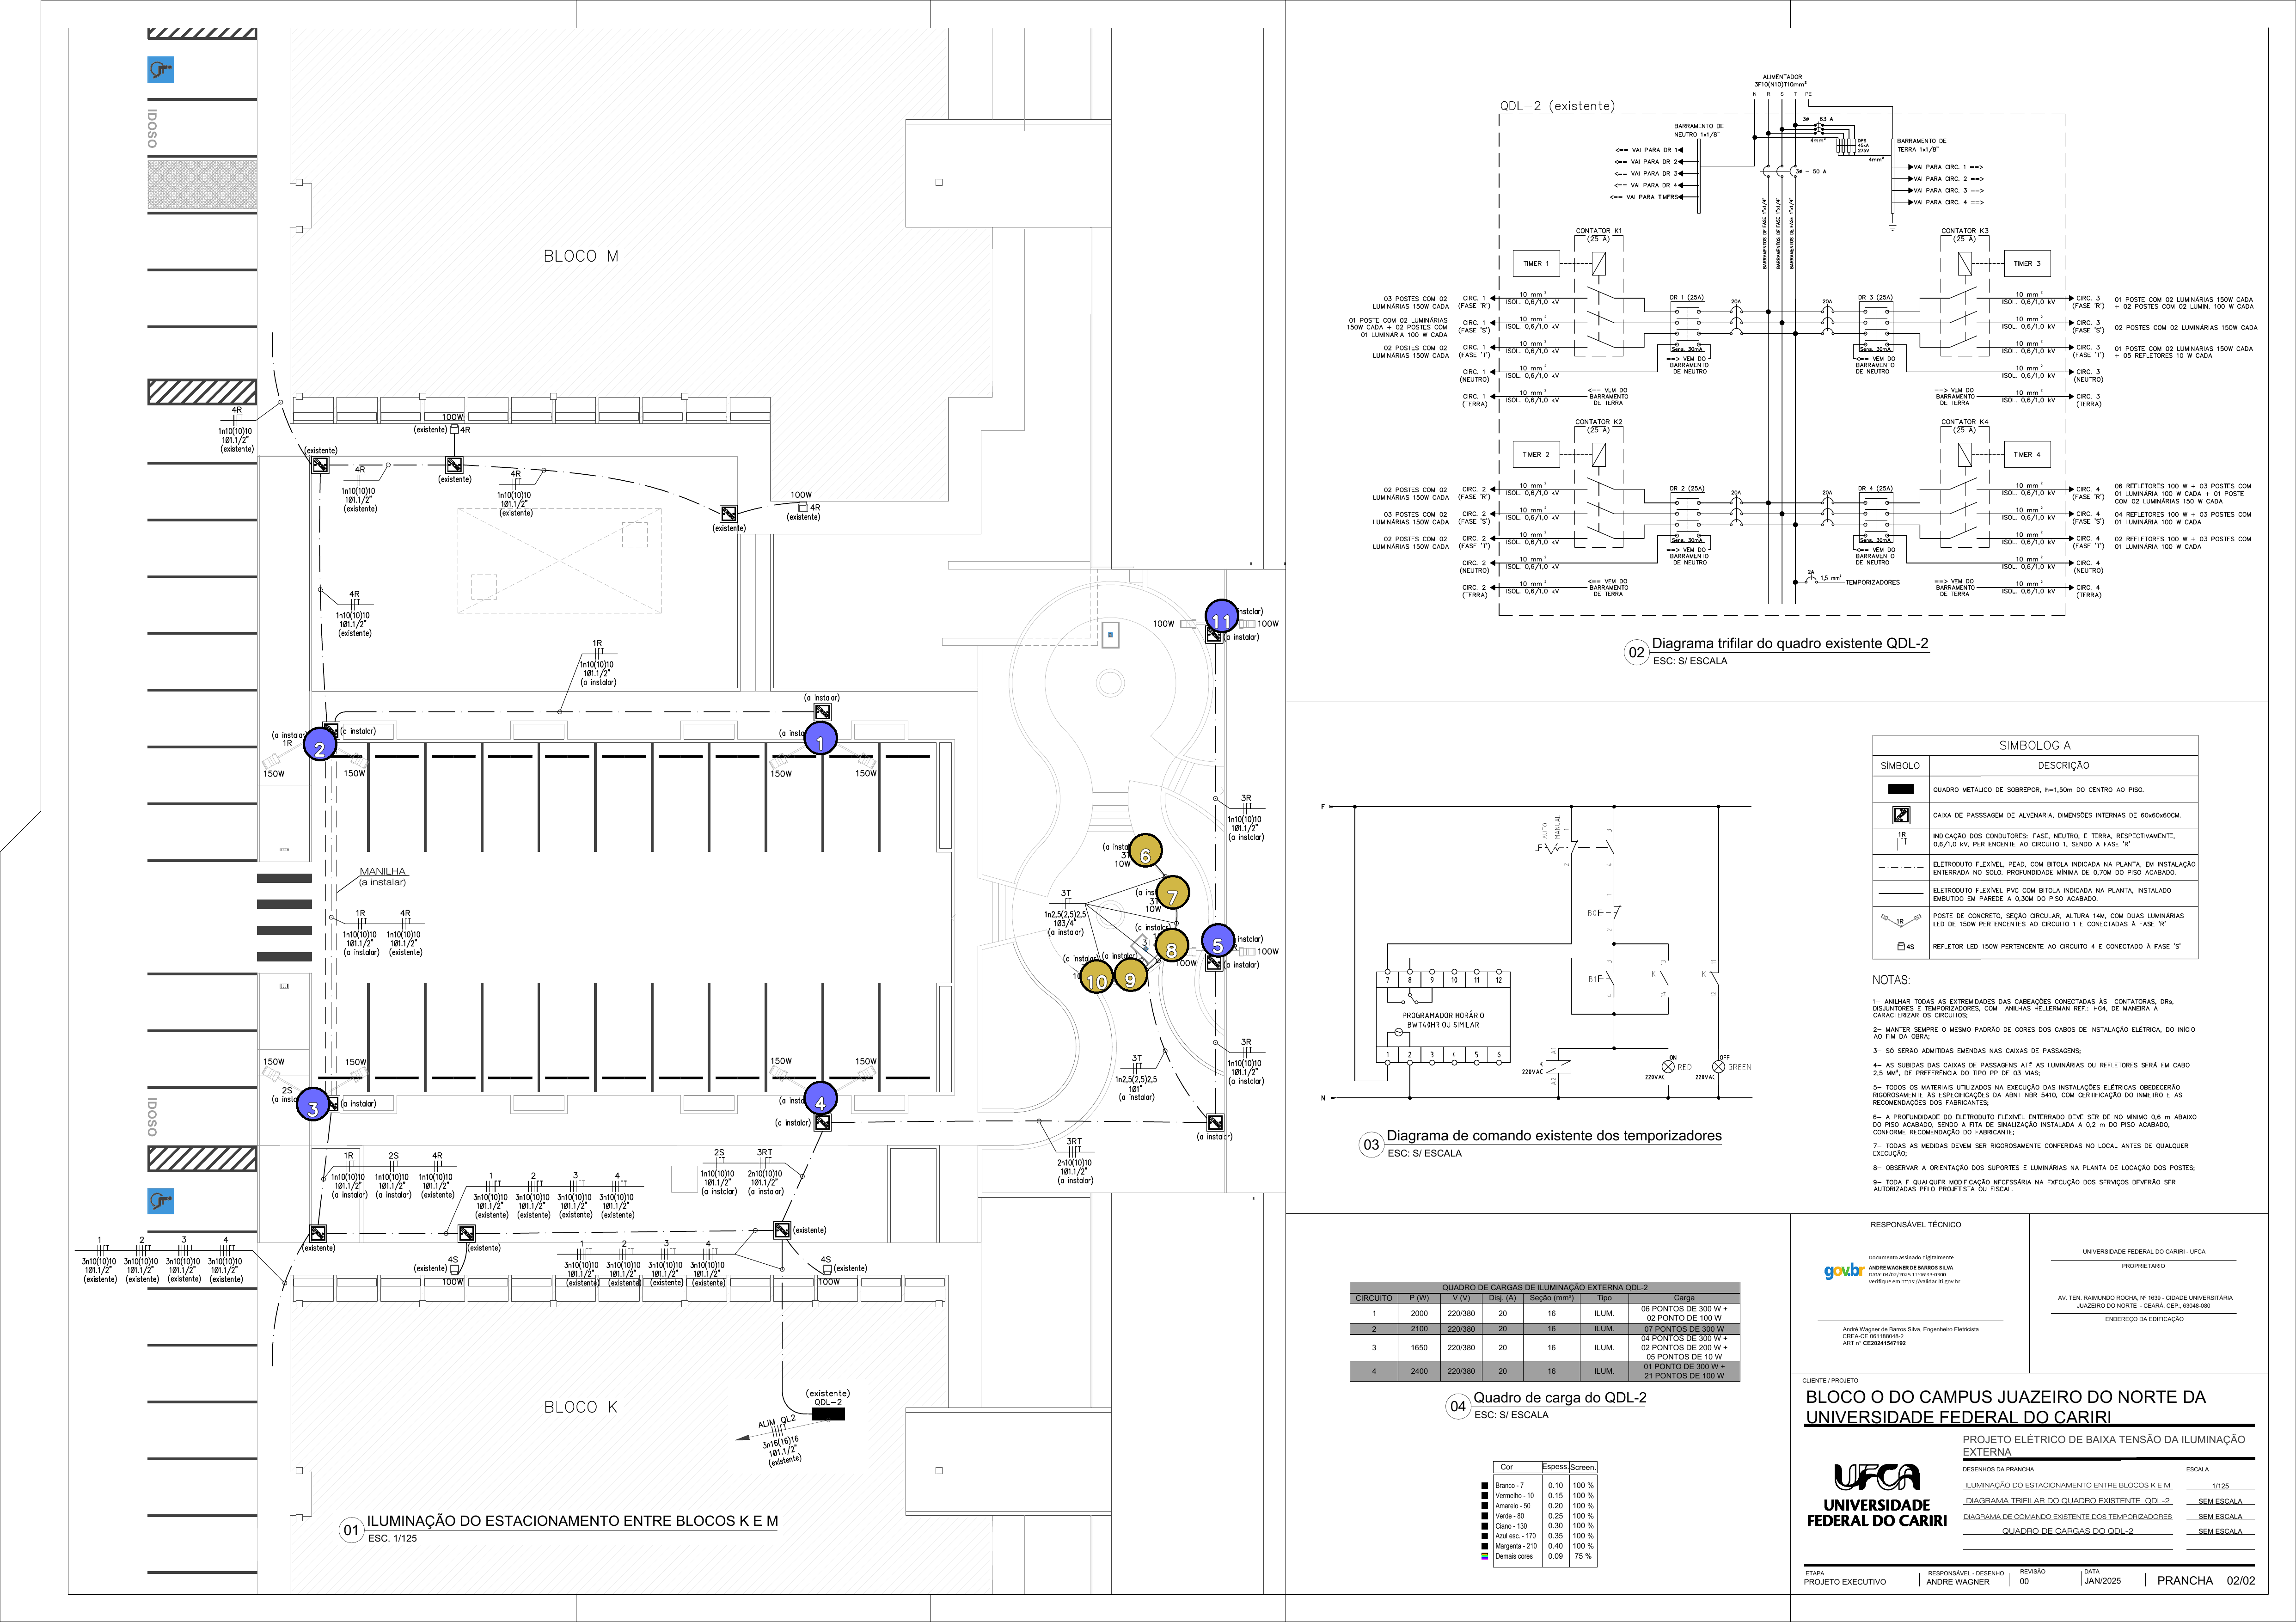
\includegraphics[width=0.95\textwidth]{pagina_11_marcado.png}
\end{figure}

\pagebreak

\subsection{Planta Página 13 - Ar Condicionado}
\begin{figure}[h!]
\centering
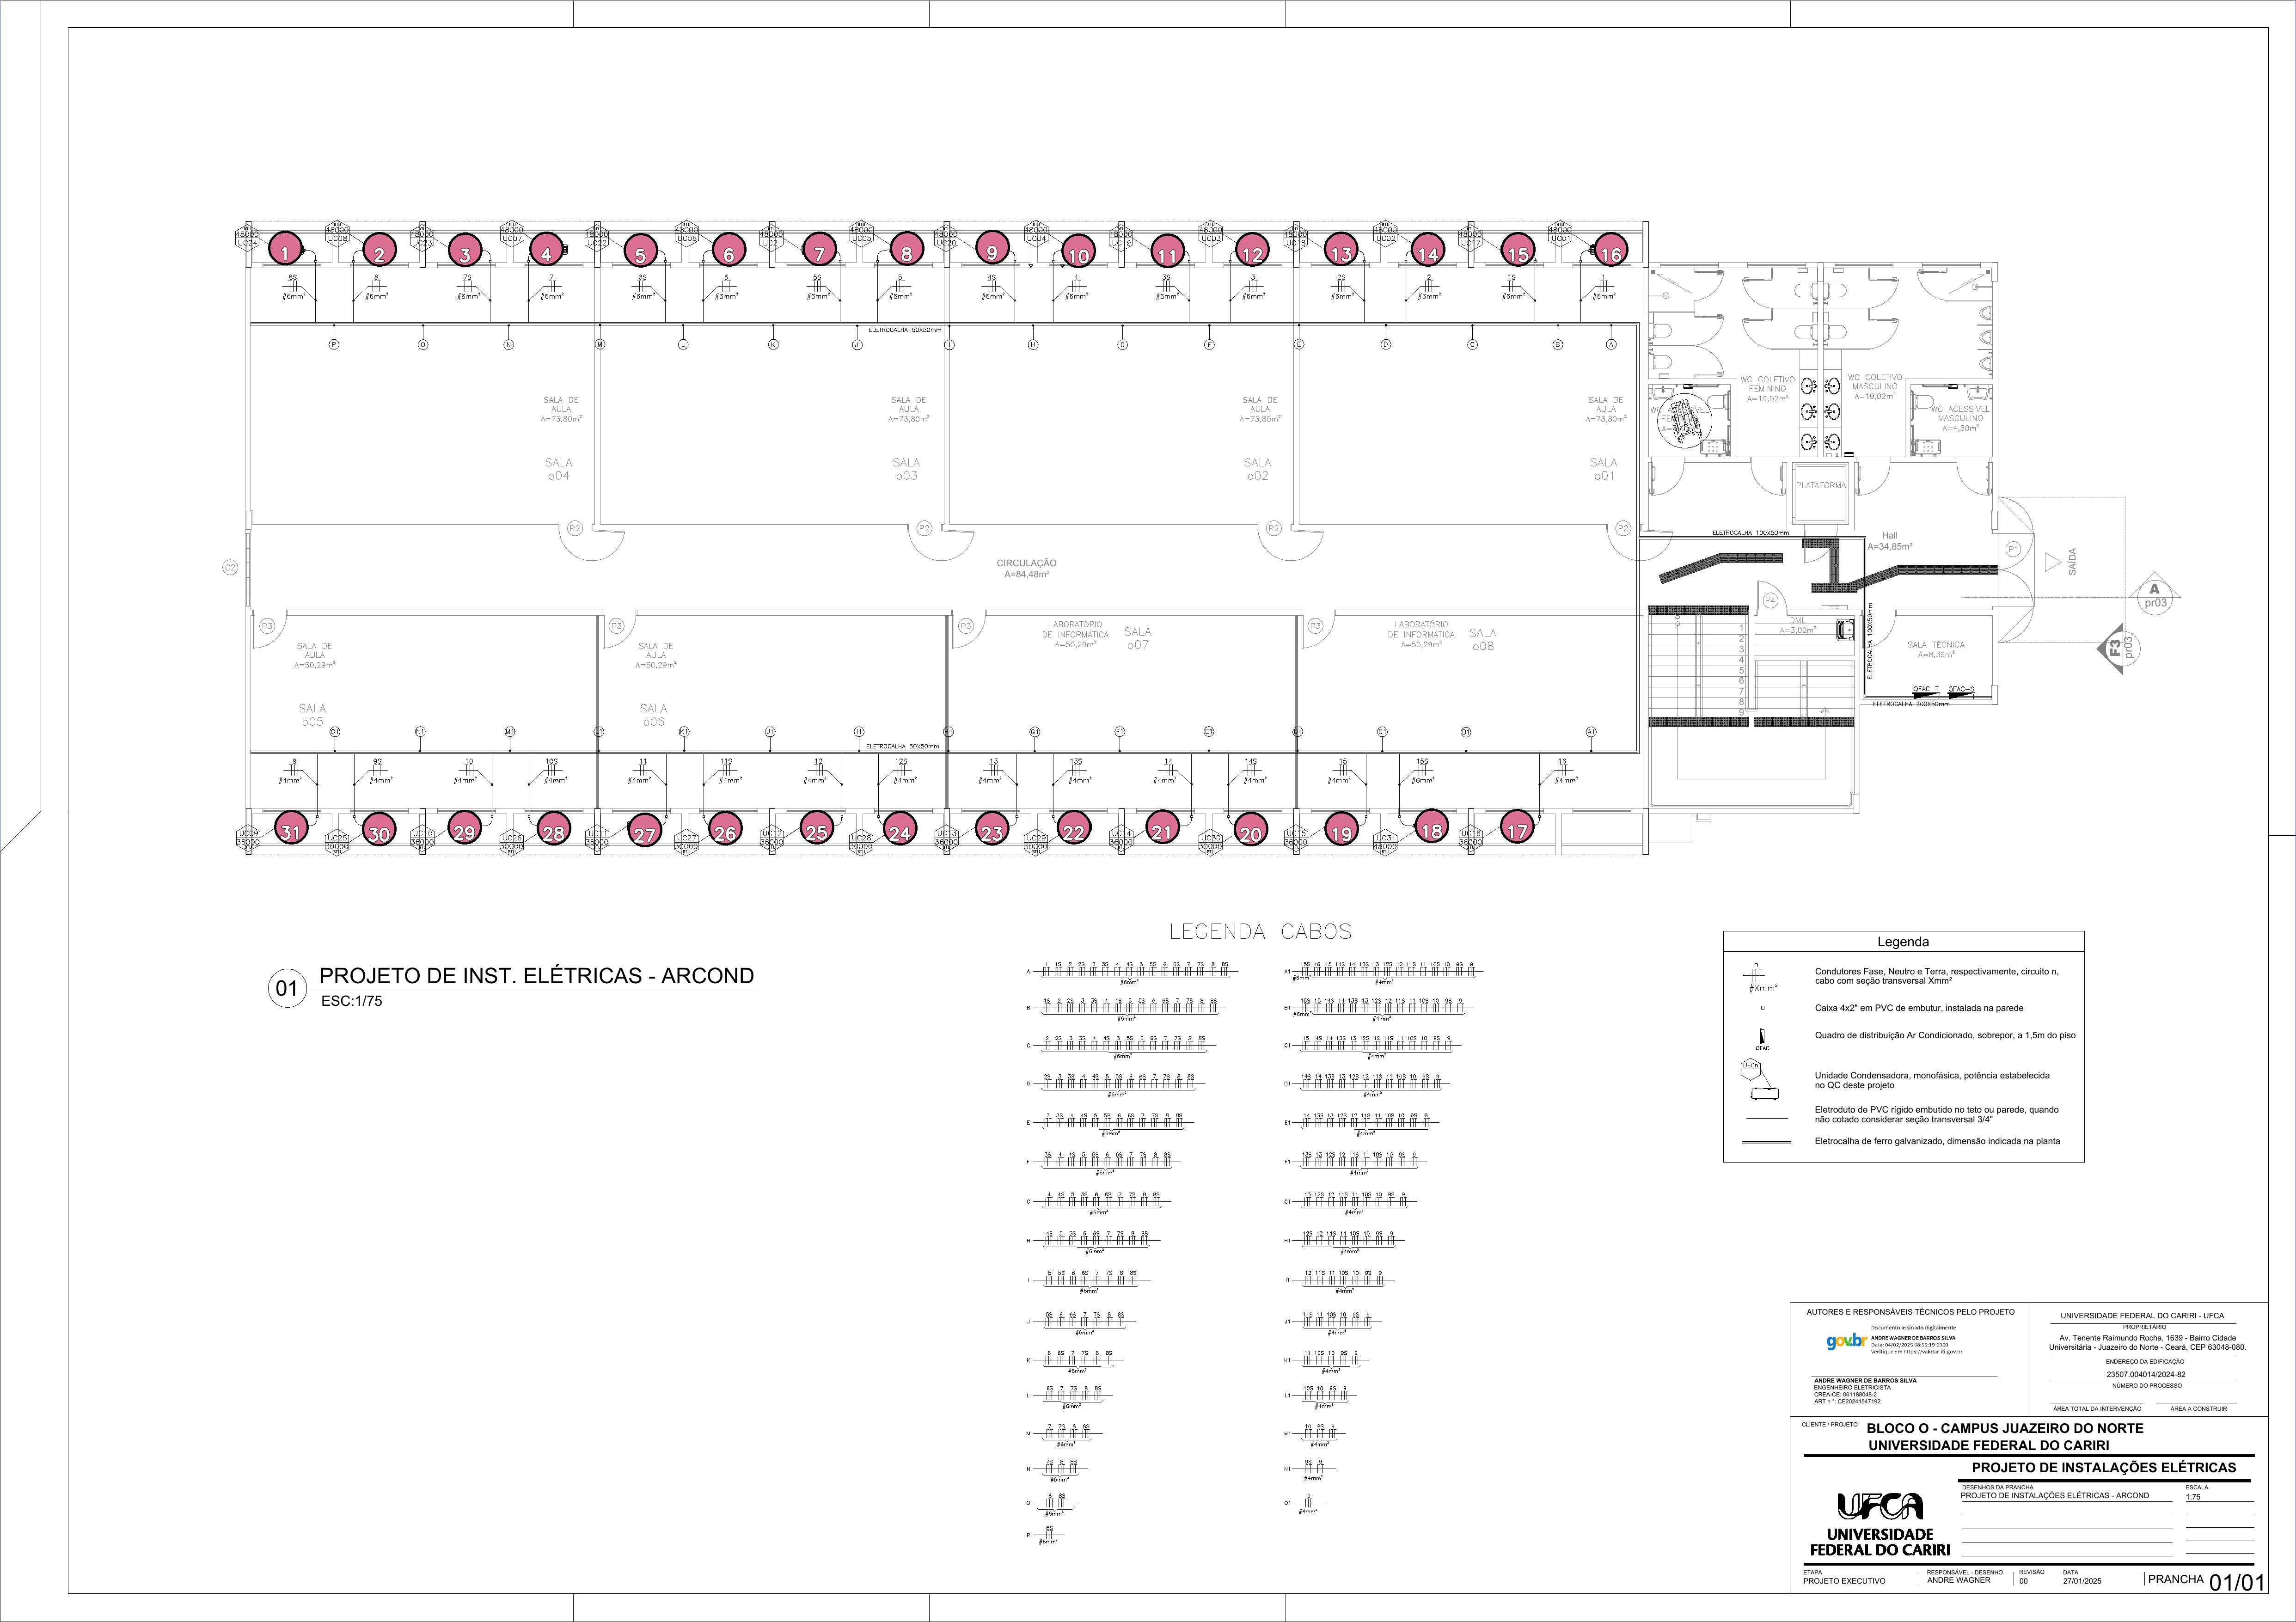
\includegraphics[width=0.95\textwidth]{pagina_13_marcado.png}
\end{figure}

\end{document}
